\documentclass[11pt, a4paper]{article}

\usepackage{fontspec}
\setmainfont{Georgia}
\setmonofont[Scale=0.85]{Menlo}

\usepackage[top=2.5cm, bottom=2.5cm, left=2.8cm, right=2.8cm]{geometry}
\usepackage{microtype}
\usepackage{parskip}
\setlength{\parskip}{6pt}

\usepackage[dvipsnames,table]{xcolor}
\definecolor{bmlblue}{RGB}{0,72,144}
\definecolor{boxbg}{RGB}{242,246,252}
\definecolor{codefg}{RGB}{30,30,50}
\definecolor{codebg}{RGB}{248,248,252}
\definecolor{rulecolor}{RGB}{180,200,230}
\definecolor{warnyellow}{RGB}{255,248,220}
\definecolor{warnborder}{RGB}{204,153,0}
\definecolor{greenbg}{RGB}{240,252,240}
\definecolor{greenborder}{RGB}{80,160,80}
\definecolor{redbg}{RGB}{255,245,245}
\definecolor{redborder}{RGB}{180,60,60}
\definecolor{glossbg}{RGB}{250,248,240}

\usepackage{amsmath, amssymb, mathtools}

\usepackage{tikz}
\usetikzlibrary{shapes.geometric, arrows.meta, positioning, fit, backgrounds, calc, decorations.pathreplacing}
\usepackage{graphicx}
\usepackage{float}

\usepackage{booktabs}
\usepackage{tabularx}
\usepackage{longtable}
\usepackage{array}
\newcolumntype{L}[1]{>{\raggedright\arraybackslash}p{#1}}
\newcolumntype{C}[1]{>{\centering\arraybackslash}p{#1}}

\usepackage{listings}
\lstdefinestyle{matlab}{
  language=Matlab,
  backgroundcolor=\color{codebg},
  basicstyle=\ttfamily\small\color{codefg},
  keywordstyle=\color{bmlblue}\bfseries,
  commentstyle=\color{gray}\itshape,
  stringstyle=\color{Maroon},
  numbers=left, numberstyle=\tiny\color{gray}, numbersep=8pt,
  frame=single, framerule=0.4pt, rulecolor=\color{rulecolor},
  breaklines=true, captionpos=b, showstringspaces=false,
  tabsize=2, xleftmargin=16pt, xrightmargin=4pt,
}
\lstdefinestyle{plain}{
  backgroundcolor=\color{codebg},
  basicstyle=\ttfamily\small\color{codefg},
  frame=single, framerule=0.4pt, rulecolor=\color{rulecolor},
  breaklines=true, xleftmargin=16pt, xrightmargin=4pt, numbers=none,
}

\usepackage{titlesec}
\titleformat{\section}{\Large\bfseries\color{bmlblue}}{}{0em}{}[\color{bmlblue}\titlerule]
\titleformat{\subsection}{\large\bfseries\color{bmlblue!80}}{}{0em}{}
\titleformat{\subsubsection}{\normalsize\bfseries\color{bmlblue!60}}{}{0em}{}

\usepackage{fancyhdr}
\pagestyle{fancy}
\fancyhf{}
\fancyhead[L]{\small\color{gray}BML Toolbox}
\fancyhead[R]{\small\color{gray}Synchronization Guide}
\fancyfoot[C]{\small\color{gray}\thepage}
\renewcommand{\headrulewidth}{0.4pt}

\usepackage[colorlinks=true, linkcolor=bmlblue, urlcolor=bmlblue]{hyperref}

\usepackage{tcolorbox}
\tcbuselibrary{skins, breakable}
\newtcolorbox{notebox}{colback=boxbg, colframe=bmlblue!40, arc=3pt,
  left=8pt, right=8pt, top=4pt, bottom=4pt, breakable}
\newtcolorbox{warnbox}{colback=warnyellow, colframe=warnborder, arc=3pt,
  left=8pt, right=8pt, top=4pt, bottom=4pt, breakable}
\newtcolorbox{greenbox}{colback=greenbg, colframe=greenborder, arc=3pt,
  left=8pt, right=8pt, top=4pt, bottom=4pt, breakable}
\newtcolorbox{redbox}{colback=redbg, colframe=redborder, arc=3pt,
  left=8pt, right=8pt, top=4pt, bottom=4pt, breakable}
\newtcolorbox{formulabox}[1][]{
  colback=boxbg, colframe=bmlblue, arc=3pt,
  left=10pt, right=10pt, top=6pt, bottom=6pt,
  title=#1, fonttitle=\bfseries\color{white},
  attach boxed title to top left={yshift=-2mm, xshift=6mm},
  boxed title style={colback=bmlblue, arc=2pt}, breakable}
\newtcolorbox{glossentry}[1]{
  colback=glossbg, colframe=bmlblue!30, arc=2pt,
  left=8pt, right=8pt, top=3pt, bottom=3pt,
  title={\small\bfseries\color{bmlblue}#1},
  attach boxed title to top left={yshift=-2mm, xshift=6mm},
  boxed title style={colback=bmlblue!15, colframe=bmlblue!30, arc=2pt},
  breakable}

\usepackage{enumitem}
\setlist[itemize]{itemsep=2pt, topsep=4pt}
\setlist[enumerate]{itemsep=2pt, topsep=4pt}
\usepackage{caption}
\captionsetup{font=small, labelfont=bf}

% ============================================================================
\begin{document}
% ============================================================================

\begin{titlepage}
\begin{tikzpicture}[remember picture, overlay]
  \fill[bmlblue] (current page.north west) rectangle ([yshift=-6cm]current page.north east);
  \node[anchor=north, text=white, font=\fontsize{28}{34}\bfseries, text width=14cm, align=center]
    at ([yshift=-1.2cm]current page.north) {BML Toolbox};
  \node[anchor=north, text=white!80, font=\fontsize{18}{24}\selectfont, text width=14cm, align=center]
    at ([yshift=-3.0cm]current page.north) {Synchronization \& Annotation System};
  \node[anchor=north, text=white!60, font=\fontsize{12}{16}\selectfont, text width=14cm, align=center]
    at ([yshift=-4.5cm]current page.north) {Complete technical guide --- Brain Modulation Laboratory};
\end{tikzpicture}
\vspace*{7cm}
\begin{center}
{\large\bfseries\color{bmlblue} Brain Modulation Laboratory}\\[4pt]
{\normalsize Massachusetts General Hospital · University of Pittsburgh}\\[12pt]
{\small\color{gray} April 2026}\\[24pt]
\hrule height 0.4pt
\vspace{8pt}
{\small\color{gray}
Covers: ROI tables · analog sync (Ripple/Zoom) · event sync (NeuroOmega, Psychtoolbox)\\
Old vs.\ new DP matching · consolidation · glossary · complete worked examples}
\end{center}
\end{titlepage}

\tableofcontents
\newpage

% ============================================================================
\section{Glossary of Key Terms}
\label{sec:glossary}
% ============================================================================

This section defines every term used throughout the document. Read this first; refer back to it any time a term is unclear.

\begin{glossentry}{Annotation table}
A standard MATLAB \texttt{table} with mandatory columns \texttt{id}, \texttt{starts}, \texttt{ends}, \texttt{duration}. The universal data structure in BML for representing any time-stamped event or segment --- stimulus onsets, recording intervals, sync events, etc. Created and enforced by \texttt{bml\_annot\_table()}.
\end{glossentry}

\begin{glossentry}{ROI table (Region of Interest)}
An annotation table extended with file-level columns: \texttt{folder}, \texttt{name}, \texttt{nSamples}, \texttt{Fs}, \texttt{filetype}, \texttt{chantype}, \texttt{s1}, \texttt{t1}, \texttt{s2}, \texttt{t2}. One row per file (or file chunk). This is the main carrier of synchronization state in the pipeline. Created by \texttt{bml\_roi\_table()}.
\end{glossentry}

\begin{glossentry}{Master / Slave}
The \textbf{master} device is the one whose clock defines ``ground truth'' time for the entire session. In BML, this is always the \textbf{Ripple/Trellis} neural recorder. All other devices are \textbf{slaves}: their sample indices must be mapped to master-clock times. The master's \texttt{warpfactor} is always 1.000000 (it is its own reference).
\end{glossentry}

\begin{glossentry}{s1, t1, s2, t2 (sync coordinates)}
Four numbers stored in every ROI table row that define a linear mapping from the file's sample indices to absolute master-clock times. \texttt{s1} and \texttt{s2} are two sample indices; \texttt{t1} and \texttt{t2} are the master-clock \emph{midpoint times} of those samples. Together they encode both a time offset and a clock-rate correction. Before synchronization, \texttt{t1}/\texttt{t2} come from OS timestamps (unreliable). After synchronization, they are true master-clock values.
\end{glossentry}

\begin{glossentry}{Sample midpoint time}
A sample at index $i$ represents the signal averaged over a window of width $1/F_s$. Its ``time'' is the midpoint of that window. If a file starts at $t_{\text{start}}$, the midpoint of its first sample is $t_{\text{start}} + 0.5/F_s$. This $\pm 0.5/F_s$ correction appears everywhere in BML and is easy to overlook.
\end{glossentry}

\begin{glossentry}{Warp factor}
The ratio between the slave device's nominal sampling rate and its effective rate as measured against the master clock. \texttt{warpfactor > 1} means the slave clock ran \emph{slow} (fewer samples per second than nominally); \texttt{warpfactor < 1} means it ran \emph{fast}. Stored per file in the ROI table. Computed as $1/ws_1$ from the time-warp model. Typical values deviate from 1 by 1--10 ppm.
\end{glossentry}

\begin{glossentry}{Clock drift}
The phenomenon where two independent crystal oscillators nominally running at the same frequency (e.g., 30\,000\,Hz) actually run at slightly different rates. A drift of 10 ppm means that after one hour, the two clocks differ by 36\,ms. Drift is corrected by the \texttt{ws1} parameter in \texttt{bml\_timewarp}, or by the \texttt{warpfactor} in event-based sync.
\end{glossentry}

\begin{glossentry}{Chunk}
A time window (defined in master time) used to subdivide a recording session for synchronization. Each chunk is synced independently, producing one row per (file $\times$ chunk) in the preliminary sync ROI. Chunking serves two purposes: (1) it limits memory usage by loading only part of each file at once, and (2) it provides multiple independent alignment estimates for the same file, which can be validated against each other during consolidation. Chunks are defined by \texttt{bml\_chunk\_sessions()}.
\end{glossentry}

\begin{glossentry}{Consolidation}
The process of merging multiple sync estimates (from different chunks of the same file, or from adjacent files of the same type) into a single, validated linear mapping per file. Think of it as fitting a ``best line'' through all the individual sync results and checking that they agree. If they do (residuals $<$ 1\,ms), the line is accepted. If they don't, an error is raised. Performed by \texttt{bml\_sync\_consolidate()}. See Section~\ref{sec:consolidate} for details.
\end{glossentry}

\begin{glossentry}{Contiguous files}
Two or more files from the same device that cover consecutive time intervals with no gap (e.g., a Zoom recorder that auto-splits into hourly files). Contiguous files share the same physical clock and can be consolidated into a single linear mapping. The boundary between them is set at the midpoint of their adjacent anchor times.
\end{glossentry}

\begin{glossentry}{Sync channel}
The physical signal used to establish synchronization. For analog sync, this is a channel present in both the master and slave recordings (e.g., a click track on Trellis \texttt{ainp1} and Zoom audio). For event sync, this is a set of discrete events simultaneously visible on both devices (e.g., TTL pulses on Trellis digital input and NeuroOmega digital input).
\end{glossentry}

\begin{glossentry}{Envelope alignment}
The coarse synchronization stage in \texttt{bml\_sync\_analog}. Both signals are processed through the analytic signal envelope (absolute value of Hilbert transform, downsampled to 100\,Hz) before cross-correlation. This produces a smooth, low-frequency representation that is robust to large time offsets ($\pm$300\,s) and polarity inversions, but has limited timing resolution ($\sim$10\,ms).
\end{glossentry}

\begin{glossentry}{LPF alignment}
The fine synchronization stage in \texttt{bml\_sync\_analog}. Both signals are low-pass filtered (4th-order zero-phase Butterworth, cutoff $\leq$4000\,Hz) and cross-correlated within a narrow scan window ($\pm$1\,s). This achieves sub-millisecond timing resolution but requires the coarse alignment to already be within the scan window.
\end{glossentry}

\begin{glossentry}{bml\_timealign}
Low-level function that finds the time offset between two continuous signals by cross-correlation. Used inside \texttt{bml\_timewarp} (and by extension \texttt{bml\_sync\_analog}) for both the envelope and LPF stages. Returns \texttt{slave\_delta\_t} and \texttt{max\_corr}.
\end{glossentry}

\begin{glossentry}{bml\_timewarp}
Low-level function that finds both the time offset \emph{and} clock drift between two continuous signals by first calling \texttt{bml\_timealign} and then running a non-linear optimization (Nelder-Mead simplex) to maximize signal correlation under a linear time-warp model. Returns new sync coordinates \texttt{(s1, t1, s2, t2, wt0, ws1)}.
\end{glossentry}

\begin{glossentry}{bml\_timealign\_annot}
Event-based alignment function. Given two sets of discrete events (as annotation tables), finds the time shift (and optionally warp) that minimizes the sum of mismatches between slave events and their nearest master counterparts. Uses brute-force scan + Nelder-Mead refinement. Used by audio and NeuroOmega sync.
\end{glossentry}

\begin{glossentry}{bml\_sync\_match\_events (DP matching)}
Event-\emph{pairing} function using dynamic programming. Unlike \texttt{bml\_timealign\_annot} (which assumes most events are paired), this function handles sequences where events may be missing on either side. It finds the optimal subset of paired events that maximizes a weighted similarity score. Used by \texttt{bml\_sync\_digital} for Psychtoolbox/task laptop sync. See Section~\ref{sec:dp} for a detailed comparison with the older approach.
\end{glossentry}

\begin{glossentry}{BIDS TSV format}
The Brain Imaging Data Structure tab-separated format for event logs. Columns: \texttt{onset} (seconds from session start) and \texttt{duration}. BML reads these via \texttt{bml\_annot\_read\_tsv()}, which auto-renames \texttt{onset} $\to$ \texttt{starts} and computes \texttt{ends = starts + duration}.
\end{glossentry}

\begin{glossentry}{Trellis / Ripple}
The master neural recorder used in the lab. Trellis is the software; Ripple is the hardware brand. The Ripple system records ECoG, LFP, and analog/digital auxiliary channels. Its file format (\texttt{.nev} for events, \texttt{.ns*} for continuous data) is read by the NPMK library. In BML, \texttt{filetype = 'trellis'}.
\end{glossentry}

\begin{glossentry}{NeuroOmega}
A microelectrode recording system (Alpha Omega) used for intraoperative MER recordings. Records neural signals and digital events in proprietary \texttt{.mat} files. Synchronized to Trellis via shared digital trigger pulses using \texttt{bml\_sync\_neuroomega\_event()}.
\end{glossentry}

\begin{glossentry}{Zoom}
A portable audio recorder (Zoom H-series) used to capture speech and a sync click track. Synchronized to Trellis either via a shared analog channel (\texttt{bml\_sync\_analog}) or via peak detection (\texttt{bml\_sync\_audio\_event}).
\end{glossentry}

\newpage
% ============================================================================
\section{System Overview and Data Flow}
\label{sec:overview}
% ============================================================================

\subsection{The synchronization problem}

A BML recording session involves up to four independent devices, each with its own clock:

\begin{center}
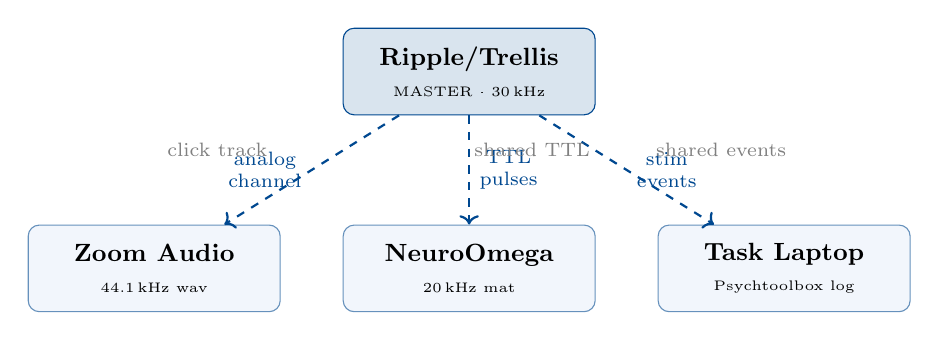
\begin{tikzpicture}[
  dev/.style={rectangle, rounded corners=4pt, draw=bmlblue!60, fill=boxbg,
              minimum width=3.2cm, minimum height=1.1cm, align=center, font=\small},
  arr/.style={->, thick, gray!70},
  sync/.style={->, thick, bmlblue, dashed}
]
  % Devices
  \node[dev, fill=bmlblue!15, draw=bmlblue] (ripple) at (0,0)
    {\textbf{Ripple/Trellis}\\{\tiny MASTER · 30\,kHz}};
  \node[dev] (zoom) at (-4, -2.5)
    {\textbf{Zoom Audio}\\{\tiny 44.1\,kHz wav}};
  \node[dev] (no) at (0, -2.5)
    {\textbf{NeuroOmega}\\{\tiny 20\,kHz mat}};
  \node[dev] (ptb) at (4, -2.5)
    {\textbf{Task Laptop}\\{\tiny Psychtoolbox log}};

  % Physical sync signals
  \draw[sync] (ripple) -- node[left, align=center, font=\scriptsize, text=bmlblue]{analog\\channel} (zoom);
  \draw[sync] (ripple) -- node[right, align=center, font=\scriptsize, text=bmlblue]{TTL\\pulses} (no);
  \draw[sync] (ripple) -- node[right, align=center, font=\scriptsize, text=bmlblue]{stim\\events} (ptb);

  % Labels
  \node[font=\scriptsize, gray] at (-3.2, -1.0) {click track};
  \node[font=\scriptsize, gray] at (0.8, -1.0) {shared TTL};
  \node[font=\scriptsize, gray] at (3.2, -1.0) {shared events};
\end{tikzpicture}
\end{center}

Each slave device's clock differs from the master by an \textbf{offset} ($\delta t$, seconds to minutes) and \textbf{drift} ($\xi$, 1--10 ppm). Both are corrected by a linear model: $t_{\text{master}} = \delta t + \xi \cdot t_{\text{slave}}$.

\subsection{Complete data flow diagram}
\label{sec:dataflow}

The diagram below shows every step from raw files to synchronized data. Boxes are functions; rounded boxes are data structures; arrows show data flow.

\begin{center}
\begin{tikzpicture}[
  node distance=0.45cm and 1.2cm,
  fn/.style={rectangle, rounded corners=3pt, draw=bmlblue!60, fill=boxbg,
             text width=4.8cm, align=center, inner sep=5pt, font=\small},
  data/.style={rectangle, rounded corners=8pt, draw=gray!60, fill=gray!8,
               text width=4.5cm, align=center, inner sep=5pt, font=\small\itshape},
  arr/.style={->, thick, bmlblue!70},
  label/.style={font=\scriptsize, gray, midway},
  grp/.style={draw=gray!40, fill=gray!5, rounded corners=6pt, inner sep=8pt}
]

% ---- Column A: ROI building ----
\node[data] (rawfiles) {Raw files on disk\\(Trellis, Zoom, NeuroOmega,\\Psychtoolbox log)};
\node[fn, below=0.5cm of rawfiles] (inforaw) {\texttt{bml\_info\_raw()}\\scan files, read OS timestamps};
\node[fn, below=0.4cm of inforaw] (roitable) {\texttt{bml\_roi\_table()}\\add default s1,t1,s2,t2};
\node[data, below=0.4cm of roitable] (roi0) {Initial ROI table\\s1=1, t1=starts+0.5/Fs\\(unreliable OS times)};
\node[fn, below=0.4cm of roi0] (chunks) {\texttt{bml\_chunk\_sessions()}\\split session into windows};
\node[data, below=0.4cm of chunks] (chunkstbl) {chunks table\\\relax[52310--52410], [52410--52510],~\ldots};

\draw[arr] (rawfiles) -- (inforaw);
\draw[arr] (inforaw) -- (roitable);
\draw[arr] (roitable) -- (roi0);
\draw[arr] (roi0) -- (chunks);
\draw[arr] (chunks) -- (chunkstbl);

% ---- Column B: Analog sync (left branch) ----
\node[fn, right=1.4cm of roi0] (syncanal) {\texttt{bml\_sync\_analog()}\\Trellis + Zoom};
\node[fn, below=0.3cm of syncanal] (timewarpenv) {\texttt{bml\_timewarp()}\\envelope, ±300 s};
\node[fn, below=0.3cm of timewarpenv] (timewarplpf) {\texttt{bml\_timewarp()}\\LPF, ±1 s};
\node[data, below=0.3cm of timewarplpf] (sroi_anal) {sync\_roi (analog)\\t1,t2 updated, warpfactor};

\draw[arr] (roi0.east) -- ++(0.5,0) |- (syncanal.west);
\draw[arr] (chunkstbl.east) -- ++(0.5,0) |- (syncanal.west);
\draw[arr] (syncanal) -- (timewarpenv);
\draw[arr] (timewarpenv) -- (timewarplpf);
\draw[arr] (timewarplpf) -- (sroi_anal);

% ---- Column C: Event sync (right branch) ----
\node[fn, right=1.3cm of syncanal] (readevt) {\texttt{bml\_read\_event()}\\read Trellis events};
\node[data, below=0.3cm of readevt] (masterevt) {master\_events\\annotation table (Trellis time)};
\node[fn, below=0.3cm of masterevt] (syncno) {\texttt{bml\_sync\_neuroomega\_event()}};
\node[fn, below=0.3cm of syncno] (syncptb) {\texttt{bml\_sync\_digital()}\\(Psychtoolbox)};
\node[data, below=0.3cm of syncptb] (sroi_evt) {sync\_roi (events)\\t1,t2 updated};

\draw[arr] (roi0.east) -- ++(1.1,0) |- (readevt.west);
\draw[arr] (readevt) -- (masterevt);
\draw[arr] (masterevt) -- (syncno);
\draw[arr] (masterevt) -- (syncptb);
\draw[arr] (syncno) -- (sroi_evt);
\draw[arr] (syncptb) -- (sroi_evt);

% ---- Consolidation row ----
\node[fn, below=1.8cm of sroi_anal, xshift=1.6cm] (consol) {\texttt{bml\_sync\_consolidate()}\\Level 1: per-file polyfit\\Level 2: contiguous files};
\node[data, below=0.4cm of consol] (finalroi) {\textbf{Final sync\_roi}\\1 row/file · validated $<$1\,ms\\all t1,t2 on Trellis clock};

\draw[arr] (sroi_anal) -- (consol);
\draw[arr] (sroi_evt.south) |- (consol.east);
\draw[arr] (consol) -- (finalroi);

% ---- Downstream ----
\node[fn, below=0.4cm of finalroi] (downstream) {\texttt{bml\_idx2time()} / \texttt{bml\_time2idx()}\\all analysis uses master time};
\draw[arr] (finalroi) -- (downstream);

\end{tikzpicture}
\end{center}

% ============================================================================
\section{Annotation Tables and the ROI Structure}
% ============================================================================

\subsection{Annotation table schema}

Every annotation table is created by \texttt{bml\_annot\_table()} which enforces the schema:

\begin{center}
\begin{tabular}{L{2.4cm} L{1.8cm} L{9.3cm}}
\toprule
\textbf{Column} & \textbf{Type} & \textbf{Description} \\
\midrule
\texttt{id} & integer & Auto-assigned by sorting on \texttt{starts}. Not stable across calls. \\
\texttt{starts} & double (s) & Start time in seconds from midnight \\
\texttt{ends} & double (s) & End time in seconds from midnight \\
\texttt{duration} & double (s) & Always \texttt{ends - starts}; never set manually \\
\emph{user cols} & any & Preserved after the core four \\
\bottomrule
\end{tabular}
\end{center}

\subsection{ROI table: the sync state carrier}

\begin{center}
\begin{tabular}{L{2.4cm} L{1.8cm} L{9.3cm}}
\toprule
\textbf{Column} & \textbf{Type} & \textbf{Description} \\
\midrule
\texttt{folder, name} & string & File location \\
\texttt{nSamples, Fs} & num & File length and nominal sample rate \\
\texttt{filetype} & string & \texttt{'trellis'}, \texttt{'zoom'}, \texttt{'neuroomega'}, \ldots \\
\texttt{chantype} & string & \texttt{'analog'}, \texttt{'digital'}, \texttt{'all'} \\
\midrule
\texttt{s1} & integer & First reference sample index \\
\texttt{t1} & double (s) & Master-clock midpoint time of sample \texttt{s1} \\
\texttt{s2} & integer & Second reference sample index \\
\texttt{t2} & double (s) & Master-clock midpoint time of sample \texttt{s2} \\
\midrule
\texttt{warpfactor} & double & $1/ws_1$; 1 = no drift \\
\texttt{chunk\_id} & integer & Which chunk produced this row \\
\texttt{sync\_type} & string & \texttt{'master'} or \texttt{'slave'} \\
\bottomrule
\end{tabular}
\end{center}

\subsection{Key annotation manipulation functions}

\begin{longtable}{L{4cm} L{10cm}}
\toprule \textbf{Function} & \textbf{What it does} \\ \midrule \endhead
\texttt{bml\_annot\_table(x)} & Constructor. Enforces schema, sorts, assigns \texttt{id}, computes \texttt{duration}. \\[2pt]
\texttt{bml\_annot\_overlap} & Returns all row pairs with overlapping intervals. \\[2pt]
\texttt{bml\_annot\_intersect} & Set intersection: intervals where x and y overlap, merged columns. \\[2pt]
\texttt{bml\_annot\_union} & Concatenate and consolidate touching/overlapping intervals. \\[2pt]
\texttt{bml\_annot\_difference} & Subtract y's time regions from x. \\[2pt]
\texttt{bml\_annot\_filter} & Keep only rows of \texttt{a} that intersect filter \texttt{f}. \\[2pt]
\texttt{bml\_annot\_consolidate} & Merge contiguous/overlapping rows (run-length encode). \\[2pt]
\texttt{bml\_annot\_extend} & Shift \texttt{starts -= ext1}, \texttt{ends += ext2} (temporal buffers). \\[2pt]
\texttt{bml\_annot\_read\_tsv} & Read BIDS TSV event logs; renames \texttt{onset}$\to$\texttt{starts}. \\[2pt]
\texttt{bml\_roi\_confluence} & Set midpoint junction times between adjacent file chunks. \\
\bottomrule
\end{longtable}

% ============================================================================
\section{The Coordinate System}
\label{sec:coords}
% ============================================================================

\subsection{Why two points?}

A single time offset $\delta t$ corrects when a recording started but not how fast its clock ran. Two reference points $(s_1, t_1)$ and $(s_2, t_2)$ encode \emph{both}: the slope of the line through them gives the effective rate; the intercept gives the offset.

\begin{center}
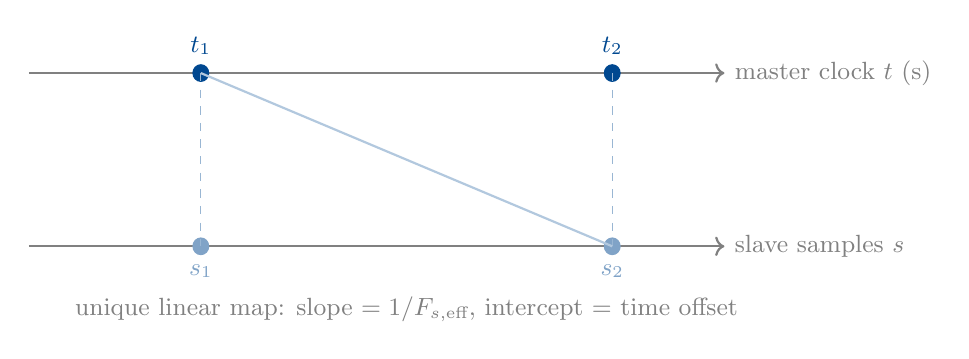
\begin{tikzpicture}[xscale=0.95]
  \draw[->, thick, gray] (-0.3,0) -- (9,0) node[right]{\small master clock $t$ (s)};
  \draw[->, thick, gray] (-0.3,-2.2) -- (9,-2.2) node[right]{\small slave samples $s$};
  \filldraw[bmlblue] (2,0) circle (3pt) node[above=3pt]{\small $t_1$};
  \filldraw[bmlblue] (7.5,0) circle (3pt) node[above=3pt]{\small $t_2$};
  \filldraw[bmlblue!50] (2,-2.2) circle (3pt) node[below=3pt]{\small $s_1$};
  \filldraw[bmlblue!50] (7.5,-2.2) circle (3pt) node[below=3pt]{\small $s_2$};
  \draw[dashed, bmlblue!40] (2,0) -- (2,-2.2);
  \draw[dashed, bmlblue!40] (7.5,0) -- (7.5,-2.2);
  \draw[bmlblue!30, thick] (2,0) -- (7.5,-2.2);
  \node[gray, font=\small] at (4.75,-3.0){unique linear map: slope $= 1/F_{s,\text{eff}}$, intercept = time offset};
\end{tikzpicture}
\end{center}

\begin{formulabox}[Index-to-time (\texttt{bml\_idx2time})]
$F_{s,\text{eff}} = (s_2-s_1)/(t_2-t_1)$\qquad
$t(i) = i/F_{s,\text{eff}} - 0.5/F_{s,\text{eff}} + (s_2 t_1 - t_2 s_1)/(s_2-s_1)$
\end{formulabox}

\begin{formulabox}[Time-to-index (\texttt{bml\_time2idx})]
$i = \mathrm{round}\!\left((t_2 s_1 - s_2 t_1 + (s_2-s_1)\,t)\,/\,(t_2-t_1)\right)$
\end{formulabox}

\textbf{Before sync}: $F_{s,\text{eff}} = F_s$ (nominal), intercept from OS timestamp (seconds off).\\
\textbf{After sync}: $t_1,t_2$ are true master-clock values; $F_{s,\text{eff}}$ may differ slightly from $F_s$.

% ============================================================================
\section{Building the Initial ROI Table}
% ============================================================================

\begin{lstlisting}[style=matlab, caption={Step 1: scan files and build the initial ROI}]
% bml_info_raw scans the directory and reads OS file metadata
cfg = [];
cfg.folder   = '/data/patient_001/session_01';
cfg.filetype = {'trellis','zoom','neuroomega'};
info = bml_info_raw(cfg);
% info: starts = file_modification_time - nSamples/Fs
%       ends   = file_modification_time  (from OS, unreliable ±seconds)

% bml_roi_table adds default sync coordinates
roi = bml_roi_table(info);
%   s1 = 1
%   t1 = starts + 0.5/Fs   (midpoint of first sample -- from OS time)
%   s2 = nSamples
%   t2 = ends   - 0.5/Fs   (midpoint of last sample  -- from OS time)
% NOTE: t1 and t2 are WRONG until synchronization is done.
\end{lstlisting}

\begin{lstlisting}[style=matlab, caption={Step 2: define session chunks}]
session = bml_annot_table(table(52310, 52610, 'VariableNames', {'starts','ends'}));
session.session_id = 1;

chunks = bml_chunk_sessions(session, 3);   % split into 3 equal chunks
% OR: bml_chunk_sessions(session, 52450)   % split at a specific time
% OR: bml_chunk_sessions(session, [], 60)  % split into 60-second pieces

% chunks is an annotation table with columns:
%   id, starts, ends, duration, session_id, session_part
\end{lstlisting}

% ============================================================================
\section{Synchronizing Audio (Zoom) to Ripple/Trellis}
% ============================================================================

\subsection{Approach A: Shared analog channel (\texttt{bml\_sync\_analog})}

Both Trellis and Zoom record the same click track on an analog channel. \texttt{bml\_sync\_analog} finds the time shift and drift by cross-correlating these signals.

\begin{lstlisting}[style=matlab]
sync_channels = table( ...
  {'trellis'; 'zoom'}, {'ainp1'; 'Ch1'}, {'analog'; 'analog'}, ...
  'VariableNames', {'filetype','channel','chantype'});
sync_channels.threshold = [NaN; NaN];  % NaN = no saturation zeroing

cfg_analog = [];
cfg_analog.roi             = roi(ismember(roi.filetype,{'trellis','zoom'}), :);
cfg_analog.chunks          = chunks;
cfg_analog.master_filetype = 'trellis';
cfg_analog.sync_channels   = sync_channels;
cfg_analog.timewarp        = true;
cfg_analog.env_scan        = 300;    % coarse: ±300 s envelope xcorr
cfg_analog.lpf_scan        = 1;     % fine:   ±1 s LPF xcorr
cfg_analog.lpf_max_freq    = 4000;
cfg_analog.chunk_extend    = 5;     % load 5 s extra each side
sync_roi_analog = bml_sync_analog(cfg_analog);
\end{lstlisting}

\subsubsection{Inside \texttt{bml\_sync\_analog}: per-chunk pipeline}

For each chunk $k$, for each slave filetype:

\begin{enumerate}
  \item \textbf{Load} master sync channel (\texttt{ainp1}) and slave sync channel (\texttt{Ch1}) as \texttt{FT\_DATATYPE\_RAW}.
  \item \textbf{Coarse alignment} --- envelope warp (lines 322--327):
\begin{lstlisting}[style=matlab]
cfg.method = 'envelope'; cfg.env_freq = 100; cfg.scan = 300;
cfg.penalty_wt0_min = 1e-3; cfg.penalty_ws1 = 1e-3;
wc_env = bml_timewarp(cfg, master, slave);
slave.time{1} = bml_idx2time(wc_env, 1:length(slave.time{1}));
\end{lstlisting}
  \item \textbf{Fine alignment} --- LPF warp (lines 338--348):
\begin{lstlisting}[style=matlab]
cfg.method = 'low-pass-filter'; cfg.scan = 1;
cfg.lpf_freq = min([master.fsample, slave.fsample, 4000]);
cfg.penalty_wt0_min = 1e-6; cfg.penalty_ws1 = 1e-4;
wc_lpf = bml_timewarp(cfg, master, slave);
slave.time{1} = bml_idx2time(wc_lpf, 1:length(slave.time{1}));
\end{lstlisting}
  \item \textbf{Write output row} (lines 352--367):
\begin{lstlisting}[style=matlab]
row.t1         = bml_idx2time(wc_lpf, slave_map.raw1); % true master-clock times
row.t2         = bml_idx2time(wc_lpf, slave_map.raw2);
row.starts     = row.t1 - 0.5 ./ row.Fs;
row.ends       = row.t2 + 0.5 ./ row.Fs;
row.warpfactor = wc_env.ws1 * wc_lpf.ws1;  % combined warp from both stages
\end{lstlisting}
\end{enumerate}

\subsection{Approach B: Digital triggers via audio-peak detection (\texttt{bml\_sync\_audio\_event})}

Approach A requires both devices to record the same \emph{continuous} analog waveform. Approach B does not: Ripple/Trellis logs the TTL click pulses as \textbf{digital events} (integers in its event channel), and the Zoom recorder captures the same pulses acoustically as amplitude peaks. \texttt{bml\_sync\_audio\_event} detects those peaks with \texttt{findpeaks} and matches them to the Trellis digital event log. This is functionally the \emph{digital} counterpart of Approach~A, and is labelled \texttt{sync\_channel='digital'} in the output table.

\begin{notebox}
  \textbf{When to use each approach.}
  Use Approach A (analog) when both devices record the sync channel as a waveform: it is more robust because it exploits the full signal shape, not just peak positions.
  Use Approach B (digital peaks) when the Zoom recording only carries a click track and there is no shared analog channel on Trellis --- the only link is the TTL events on the Ripple digital input and the acoustic peaks in the Zoom audio.
\end{notebox}

\begin{lstlisting}[style=matlab]
% master_events come from Ripple's DIGITAL event channel (TTL pulses)
master_events = bml_read_event(trellis_roi);
master_events = bml_event2annot([], master_events);
% Keep only click/sync events (e.g. value==1)
master_events = master_events(master_events.value == 1, :);

cfg = [];
cfg.roi           = roi(strcmp(roi.filetype,'zoom'), :);
cfg.master_events = master_events;   % <-- digital events from Ripple
cfg.scan          = 100;    cfg.scan_step = 0.1;
cfg.min_rph       = 0.5;    % peaks must be > 50% of file max amplitude
cfg.min_ipi       = 0.05;   % peaks must be > 50 ms apart
cfg.timewarp      = false;
cfg.diagnostic_plot = true;
sync_roi_zoom = bml_sync_audio_event(cfg);
% sync_roi_zoom.sync_channel == 'digital'
\end{lstlisting}

Per file: \texttt{findpeaks(abs(audio))} $\to$ build slave event table $\to$ \texttt{bml\_timealign\_annot} $\to$ apply shift/warp to \texttt{t1,t2}. Contiguous files averaged together.

% ============================================================================
\section{Synchronizing NeuroOmega to Ripple/Trellis}
% ============================================================================

NeuroOmega shares TTL pulse events with Trellis via a digital input. Both devices log the same physical pulses in their own clocks.

\begin{lstlisting}[style=matlab]
master_events = bml_read_event(trellis_roi);
master_events = bml_event2annot([], master_events);
master_events = master_events(strcmp(master_events.type,'STIM_ON'), :);

cfg = [];
cfg.roi           = roi(strcmp(roi.filetype,'neuroomega'), :);
cfg.master_events = master_events;
cfg.scan          = 100;   cfg.scan_step = 0.1;
cfg.coarsetol     = 100;   % restrict master events to ±100 s window
cfg.timewarp      = false; % true for sessions > 30 min
cfg.timetol       = 1e-6;
cfg.diagnostic_plot = true;
sync_roi_no = bml_sync_neuroomega_event(cfg);
\end{lstlisting}

Per file:
\begin{enumerate}
  \item \texttt{bml\_read\_event(roi(i,:))} --- read NeuroOmega events
  \item \texttt{bml\_event2annot()} --- convert to annotation table
  \item \texttt{bml\_annot\_filter(master, bml\_annot\_extend(roi(i,:), coarsetol))} --- narrow master to $\pm$100\,s window
  \item \texttt{bml\_timealign\_annot(cfg, master\_events, slave\_events)} --- find $\delta t$ (and optionally $\xi$)
  \item Update \texttt{t1,t2} via: \texttt{roi.t1 = (roi.t1 - midpt) .* warpfactor + midpt + slave\_dt}
\end{enumerate}

% ============================================================================
\section{Synchronizing Task Laptop (Psychtoolbox) to Ripple}
\label{sec:ptb}
% ============================================================================

\subsection{The setup}

A task laptop runs Psychtoolbox (or PsychoPy) and logs every stimulus onset, response, and event with its own system clock. The same task sends TTL pulses to both the Ripple digital input and the task laptop (or the laptop time-stamps events that coincide with Ripple-logged pulses). The goal is to map task laptop event times onto the Trellis master clock.

\subsection{Step 1: Read the task log file}

Task logs are typically saved as TSV or CSV files following the BIDS convention:

\begin{lstlisting}[style=matlab, caption={Reading a Psychtoolbox / BIDS event log}]
% BIDS TSV format: columns 'onset' and 'duration' (both in seconds from task start)
% bml_annot_read_tsv auto-renames 'onset' -> 'starts', computes 'ends'
ptb_events = bml_annot_read_tsv('sub-DM1001_ses-intraop_task-speech_events.tsv');
% ptb_events: id, starts, ends, duration, trial_type, response_time, ...
% starts = seconds from task start (laptop clock, NOT master clock)
\end{lstlisting}

For non-BIDS formats, build the annotation table manually:
\begin{lstlisting}[style=matlab]
raw = readtable('psychtoolbox_log.csv');
% raw has columns: onset_time, event_type, trial_id

ptb_events = bml_annot_table(table( ...
  raw.onset_time, ...          % starts (laptop clock seconds)
  raw.onset_time, ...          % ends (instantaneous events)
  'VariableNames', {'starts','ends'}));
ptb_events.type  = raw.event_type;
ptb_events.value = ones(height(ptb_events), 1);
\end{lstlisting}

\subsection{Step 2: Get the same events from Ripple}

The Ripple digital input recorded the same TTL pulses that the laptop sent (or received). Extract them:

\begin{lstlisting}[style=matlab]
master_events = bml_read_event(trellis_roi);
master_events = bml_event2annot([], master_events);
% Keep only the event type corresponding to task triggers
master_events = master_events(master_events.value == 1, :);
% master_events.starts = times in TRELLIS clock [seconds]
\end{lstlisting}

\subsection{Step 3: Synchronize with \texttt{bml\_sync\_digital}}

\begin{lstlisting}[style=matlab, caption={Synchronizing Psychtoolbox events to Trellis}]
cfg = [];
cfg.timetol        = 1e-3;   % 1 ms tolerance
cfg.sim_threshold  = 0.9;    % minimum similarity to accept a match
cfg.diagnostic_plot = true;
cfg.plot_title     = 'Psychtoolbox to Trellis';

% Weight configuration for event matching
cfg.timetol           = 1e-3;   % timing tolerance for similarity kernel
cfg.weight_time_pre   = 1/4;    % weight for pre-event interval match
cfg.weight_time_post  = 1/4;    % weight for post-event interval match
cfg.weight_value_pre  = 1/4;    % weight for pre-event value match
cfg.weight_value_post = 1/4;    % weight for post-event value match
cfg.weight_onset      = 0;      % set > 0 to prefer temporally close matches

[sync_roi_ptb, hF] = bml_sync_digital(cfg, master_events, ptb_events);
% sync_roi_ptb columns:
%   starts, ends   -- time window of matched events (in master time)
%   delta_t        -- shift to add to laptop times to get master times
%   warpfactor     -- clock rate correction (1 = no drift)
%   mean_sim       -- mean similarity score of matched event pairs
%   s1, t1, s2, t2 -- sync coordinates (from sample column if available)
\end{lstlisting}

\subsection{Step 4: Apply sync to task events}

After synchronization, convert all laptop event times to master clock:

\begin{lstlisting}[style=matlab]
% Apply the linear transformation from sync_roi_ptb
delta_t    = sync_roi_ptb.delta_t(1);
warpfactor = sync_roi_ptb.warpfactor(1);
tbar       = mean(ptb_events.starts);   % pivot for warping

ptb_events_synced = ptb_events;
ptb_events_synced.starts = (ptb_events.starts - tbar) .* warpfactor + tbar + delta_t;
ptb_events_synced.ends   = (ptb_events.ends   - tbar) .* warpfactor + tbar + delta_t;
% Now ptb_events_synced.starts are in TRELLIS (master) clock seconds
\end{lstlisting}

\subsection{Step 4b: Exact-match fallback strategy}
\label{sec:ptb_fallback}

\texttt{bml\_sync\_digital} returns a single linear model. A more precise strategy, used in production scripts, exploits the DP matching directly:

\begin{itemize}
  \item For task events that \textbf{matched a Ripple event} in the DP: substitute the exact Ripple timestamp. No interpolation error.
  \item For task events in \textbf{gaps} (no matching Ripple event --- task events the Ripple didn't log): use the linear warp as a fallback.
\end{itemize}

This hybrid approach gives sub-millisecond accuracy for most events while gracefully handling trials where the Ripple event was not recorded.

\begin{lstlisting}[style=matlab, caption={Fallback strategy: exact Ripple times where available, linear interpolation elsewhere}]
% SYNCHRONIZING EVENT FILES TO RIPPLE EVENTS
% Will inherit exact timing from Ripple. Looping through events_files.
events_files.delta_t(:)    = nan;
events_files.warpfactor(:) = nan;
events_files.n(:)          = nan;

for i = 1:height(events_files)

  % Skip if no matching Ripple (NEV) events exist for this file
  % (prevents matching pre-op events to intraop NEV files)
  nev_events_files = bml_annot_filter(roi_nev, events_files(i,:));
  if isempty(nev_events_files); continue; end

  task_events = bml_annot_read_tsv( ...
    fullfile(events_files.path{i}, events_files.filename{i}));

  % DP matching: find which task events correspond to which master events
  cfg = [];
  cfg.timetol        = 0.003;   % 3 ms timing tolerance for similarity kernel
  cfg.weight_onset   = 0.1;     % small onset weight to prefer temporally close matches
  cfg.diagnostic_plot = true;
  [idxs_master, idxs_task, mean_sim, simv] = ...
    bml_sync_match_events(cfg, master_events, task_events);

  % Find the longest contiguous block of matched pairs
  % (guards against spurious matches at session boundaries)
  disconts_idx       = [1, find(diff(idxs_master) > 3), length(idxs_master)];
  [~, cont_idx]      = max(diff(disconts_idx));
  start_idx          = disconts_idx(cont_idx) + 1;
  end_idx            = disconts_idx(cont_idx + 1) - 1;

  % Fit linear warp as FALLBACK (for events without a direct Ripple match)
  tbar = mean(task_events.starts(idxs_task), 'omitnan');
  p    = polyfit( ...
    task_events.starts(idxs_task(start_idx:end_idx))   - tbar, ...
    master_events.starts(idxs_master(start_idx:end_idx)) - tbar, 1);

  events_files.warpfactor(i) = p(1);
  events_files.delta_t(i)    = p(2);
  events_files.n(i)          = height(task_events(idxs_task, :));

  % Compute fallback times for ALL task events via the linear model
  task_events.starts_corrected = ...
    (task_events.starts - tbar) .* p(1) + tbar + p(2);

  % PRIMARY: substitute exact Ripple time for matched events
  task_events.starts = bml_map( ...
    1:height(task_events), ...
    idxs_task, master_events.starts(idxs_master), nan);

  % FALLBACK: fill gaps with linear-warp times
  task_events.starts(isnan(task_events.starts)) = ...
    task_events.starts_corrected(isnan(task_events.starts));

  % Save synchronized event file
  bml_annot_write_tsv(task_events, ...
    fullfile(PATH_ANNOT, strrep(events_files.filename{i}, '.tsv', '-sync.tsv')));

  fprintf('sync %s  delta_t=%.4f  mean_sim=%.3f  warpfactor=%.7f\n', ...
    events_files.filename{i}, p(2), mean_sim, p(1));
end
\end{lstlisting}

\begin{notebox}
  \textbf{Why two passes?}
  The linear warp corrects for clock drift globally. But Ripple's event timestamps are the \emph{ground truth}: they were recorded at hardware precision (30\,kHz sample clock). Where a direct match exists, using the Ripple timestamp is always more accurate than any interpolated value. The fallback linear model fills only the gaps.
\end{notebox}

\begin{warnbox}
  \textbf{Choosing the longest contiguous block.} The DP matching may produce a few spurious matches at the very start or end of the session (where the event sequences don't overlap well). Taking the longest contiguous block --- defined by no gap of more than 3 unmatched master events --- avoids these boundary artefacts in the linear fit.
\end{warnbox}

% ============================================================================
\section{Event Alignment: From Brute-Force to Dynamic Programming}
\label{sec:dp}
% ============================================================================

\subsection{The problem with simple event matching}

Both \texttt{bml\_sync\_audio\_event} and \texttt{bml\_sync\_neuroomega\_event} use \texttt{bml\_timealign\_annot}, which works well when:
\begin{itemize}
  \item Most slave events have a corresponding master event (few missing events)
  \item The initial OS-timestamp coarse alignment is roughly correct
\end{itemize}

But for Psychtoolbox/task events, \textbf{neither assumption may hold}:
\begin{itemize}
  \item The laptop clock can be hours off from the master
  \item Some trial types may be absent on one side
  \item The event sequence may contain events of many different values
\end{itemize}

\texttt{bml\_sync\_match\_events} solves this with dynamic programming.

\subsection{The old approach (archived, pre-2025)}

The archived version (\texttt{bml\_sync\_match\_events\_archivePLB20250715.m}) used a \textbf{4-feature} similarity function:

\begin{lstlisting}[style=matlab, caption={Old 4-feature similarity (archived)}]
% Feature vector for event i (4 features):
% [ interval_before_i, interval_after_i, value[i], value[i+1] ]
x1 = [events1_delta_starts(1:end-1), ...   % pre-interval
      events1_delta_starts(2:end),   ...   % post-interval
      events1.value(1:end-2),        ...   % pre value
      events1.value(2:end-1)];            % post value

% Similarity (old): no onset term, fixed equal weights
similarity_fun = @(x1,x2) ...
  wdt1 .* (1./(1+((x1(:,1)-x2(:,1))./timetol).^2)) + ...  % pre-interval
  wdt2 .* (1./(1+((x1(:,2)-x2(:,2))./timetol).^2)) + ...  % post-interval
  wv1  .* (x1(:,3)==x2(:,3)) + ...                         % pre-value
  wv2  .* (x1(:,4)==x2(:,4));                              % post-value
\end{lstlisting}

\textbf{Problem}: without an onset term, the algorithm had no preference for matches that are close in \emph{absolute} time. Two events with identical inter-event intervals but 1\,hour apart in the session were considered equally good candidates. In sessions with repetitive, regular event patterns, this could lead to mismatches.

\subsection{The new approach (current)}

The current version adds a \textbf{5th feature}: the absolute onset time of each event. This breaks ties by preferring pairs that are close in the session:

\begin{lstlisting}[style=matlab, caption={New 5-feature similarity (current)}]
% Feature vector for event i (5 features):
% [ pre-interval, post-interval, pre-value, post-value, ONSET TIME ]
x1 = [events1_delta_starts(1:end-1), ...
      events1_delta_starts(2:end),   ...
      events1.value(1:end-2),        ...
      events1.value(2:end-1),        ...
      events1.starts(1:end-2)];      % <-- NEW: absolute onset time

% Similarity (new): onset term with configurable weight
similarity_fun = @(x1,x2) ...
  wdt1 .* (1./(1+((x1(:,1)-x2(:,1))./timetol).^2))   + ...  % pre-interval
  wdt2 .* (1./(1+((x1(:,2)-x2(:,2))./timetol).^2))   + ...  % post-interval
  wv1  .* (x1(:,3)==x2(:,3))                          + ...  % pre-value
  wv2  .* (x1(:,4)==x2(:,4))                          + ...  % post-value
  wo   .* (1./(1+((x1(:,5)-x2(:,5))./onsettol).^2));        % <-- onset time

% All weights are normalized to sum to 1
total = wdt1 + wdt2 + wv1 + wv2 + wo;
wdt1 = wdt1/total;  % etc.
\end{lstlisting}

\subsubsection{Summary of differences}

\begin{center}
\begin{tabular}{L{4.5cm} L{4.5cm} L{4.5cm}}
\toprule
\textbf{Aspect} & \textbf{Old (archived)} & \textbf{New (current)} \\
\midrule
Features per event & 4 & 5 \\
Onset term & Absent & Present (\texttt{weight\_onset}, default 0) \\
Weight params & \texttt{weight\_time\_pre/post}, \texttt{weight\_value\_pre/post} & Same + \texttt{weight\_onset} + \texttt{onsettol} \\
Normalization & Fixed 1/4 each & Sum-normalized \\
Robustness & Can confuse repetitive patterns & Onset weight breaks ties \\
Backwards compat & --- & \texttt{weight\_onset=0} replicates old behavior \\
\bottomrule
\end{tabular}
\end{center}

Setting \texttt{cfg.weight\_onset = 0} (the default) exactly reproduces the old behavior. Setting it to a positive value (e.g., 0.5) adds a preference for temporally proximate matches, which is useful for long sessions or repetitive event patterns.

\subsection{The dynamic programming algorithm (both versions)}

The DP algorithm itself is identical in both versions --- only the similarity function differs.

\begin{center}
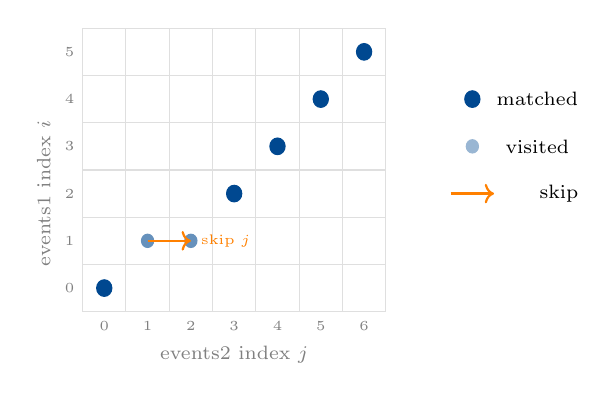
\begin{tikzpicture}[xscale=0.55, yscale=0.6]
  % Grid
  \foreach \i in {0,1,2,3,4,5} {
    \foreach \j in {0,1,2,3,4,5,6} {
      \draw[gray!25] (\j,\i) rectangle (\j+1,\i+1);
    }
  }
  % Axes labels
  \foreach \j/\lbl in {0/0,1/1,2/2,3/3,4/4,5/5,6/6}
    \node[gray, font=\tiny] at (\j+0.5, -0.3) {\lbl};
  \foreach \i/\lbl in {0/0,1/1,2/2,3/3,4/4,5/5}
    \node[gray, font=\tiny] at (-0.3, \i+0.5) {\lbl};
  \node[gray, font=\scriptsize] at (3.5, -0.9) {events2 index $j$};
  \node[gray, font=\scriptsize, rotate=90] at (-0.9, 2.5) {events1 index $i$};
  % DP path
  \foreach \i/\j in {0/0, 1/1, 1/2, 2/3, 3/4, 4/5, 5/6} {
    \filldraw[bmlblue!60] (\j+0.5, \i+0.5) circle (4pt);
  }
  % Matched pairs (diagonal steps)
  \foreach \i/\j in {0/0, 2/3, 3/4, 4/5, 5/6} {
    \filldraw[bmlblue] (\j+0.5, \i+0.5) circle (5pt);
  }
  % Skip (horizontal = skip events2 j)
  \draw[->, thick, orange] (1.5,1.5) -- (2.5,1.5) node[right, font=\tiny]{skip $j$};
  % Legend
  \filldraw[bmlblue] (9,4.5) circle (5pt); \node[font=\scriptsize] at (10.5,4.5){matched};
  \filldraw[bmlblue!40] (9,3.5) circle (4pt); \node[font=\scriptsize] at (10.5,3.5){visited};
  \draw[->,thick,orange] (8.5,2.5)--(9.5,2.5); \node[font=\scriptsize] at (11.0,2.5){skip};
\end{tikzpicture}
\end{center}

\begin{lstlisting}[style=matlab, caption={DP recurrence (same in old and new versions)}]
dp = zeros(n+1, m+1);
for i = 1:n
  for j = 1:m
    dp(i+1,j+1) = max([ ...
      dp(i,j)   + similarity_fun(x1(i,:), x2(j,:)), ... % match i to j
      dp(i+1,j),                                     ... % skip j (missing in events1)
      dp(i,j+1)  ]);                                     % skip i (missing in events2)
  end
end
% Backtrack from dp(n+1, m+1) to recover paired indices
\end{lstlisting}

This is identical in structure to the Longest Common Subsequence (LCS) algorithm, but with a continuous similarity score instead of binary match/mismatch. Skipping costs nothing (dp stays flat), while matching adds the similarity score. The backtracking recovers the set of pairs that maximises the total accumulated similarity.

\subsection{How \texttt{bml\_sync\_digital} uses the DP output}

After DP matching, \texttt{bml\_sync\_digital} fits a linear model:

\begin{lstlisting}[style=matlab]
% dtv = time differences for all matched pairs
dtv = master_events.starts(idxs_master) - slave_events.starts(idxs_slave);

% Detect contiguous high-similarity chunks
% (similarity drops when event sequences diverge)
cfg1.threshold = sim_threshold;   % default 0.9
chunks = bml_annot_detect(cfg1, sim_raw);  % segments where sim > 0.9

% For each chunk: fit linear model
for i = 1:height(chunks)
  chunk_idxs = ceil(chunks.starts(i)):floor(chunks.ends(i));
  p = polyfit(master_events.starts(idxs_master(chunk_idxs)) - tbar, ...
              dtv(chunk_idxs), 1);
  chunks.warp(i)    = p(1);
  chunks.delta_t(i) = p(2);
end

% Consolidate chunks with consistent delta_t
cfg1.criterion = @(x) (abs(max(x.delta_t) - min(x.delta_t)) < cfg.timetol);
cons_chunks = bml_annot_consolidate(cfg1, chunks);

% Final polyfit across all events in each consolidated chunk
% If slave has a 'sample' column, also compute (s1,t1,s2,t2) coordinates:
p = polyfit(slave_events.sample(idxs(chunk_idxs)), ...
            master_events.starts(idxs_master(chunk_idxs)), 1);
cons_chunks.s1(i) = slave_events.sample(idxs(chunk_idxs(1)));
cons_chunks.t1(i) = cons_chunks.s1(i) * p(1) + p(2);
cons_chunks.s2(i) = slave_events.sample(idxs(chunk_idxs(end)));
cons_chunks.t2(i) = cons_chunks.s2(i) * p(1) + p(2);
\end{lstlisting}

% ============================================================================
% ============================================================================
\section{Alignment Function Hierarchy}
\label{sec:alignment_hierarchy}
% ============================================================================

This section provides a complete map of the low-level alignment functions, how they relate to each other, and when each one is appropriate.

\subsection{Call graph}

\begin{center}
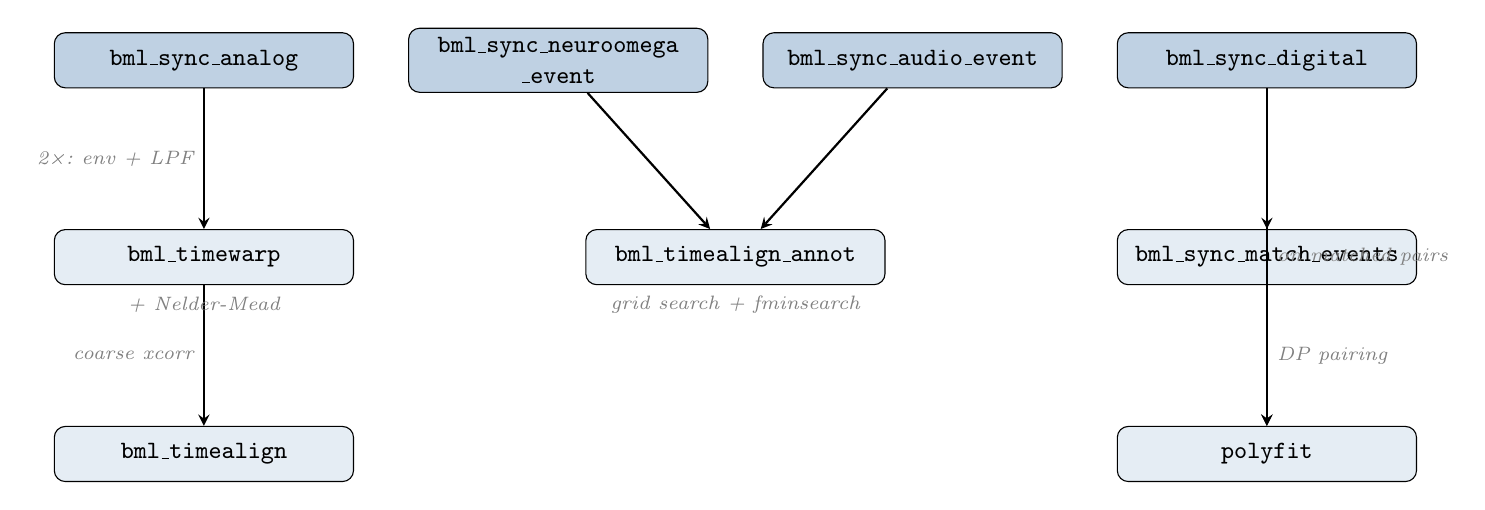
\begin{tikzpicture}[
  box/.style={draw, rounded corners, fill=bmlblue!10, minimum width=3.8cm, minimum height=0.7cm, font=\small\ttfamily, align=center},
  highbox/.style={draw, rounded corners, fill=bmlblue!25, minimum width=3.8cm, minimum height=0.7cm, font=\small\ttfamily\bfseries, align=center},
  arr/.style={->, >=stealth, thick},
  note/.style={font=\scriptsize\itshape, text=gray}
]

% High-level row
\node[highbox] (SA)  at (0,0)      {bml\_sync\_analog};
\node[highbox] (SN)  at (4.5,0)    {bml\_sync\_neuroomega\\\_event};
\node[highbox] (SAE) at (9,0)      {bml\_sync\_audio\_event};
\node[highbox] (SD)  at (13.5,0)   {bml\_sync\_digital};

% Mid-level row
\node[box] (TW)  at (0,-2.5)    {bml\_timewarp};
\node[box] (TAA) at (6.75,-2.5) {bml\_timealign\_annot};
\node[box] (SME) at (13.5,-2.5) {bml\_sync\_match\_events};

% Low-level row
\node[box] (TA)  at (0,-5)      {bml\_timealign};
\node[box] (PF)  at (13.5,-5)   {polyfit};

% Arrows high→mid
\draw[arr] (SA)  -- node[left, note]{2×: env + LPF} (TW);
\draw[arr] (SN)  -- (TAA);
\draw[arr] (SAE) -- (TAA);
\draw[arr] (SD)  -- (SME);
\draw[arr] (SD)  -- node[right, note]{on matched pairs} (PF);

% Arrows mid→low
\draw[arr] (TW)  -- node[left, note]{coarse xcorr} (TA);
\draw[arr] (SME) -- node[right, note]{DP pairing} (PF);

% Self-labels (optimization within the function)
\node[note] at (0,-3.1) {+ Nelder-Mead};
\node[note] at (6.75,-3.1) {grid search + fminsearch};

\end{tikzpicture}
\end{center}

\subsection{The two dimensions}

There are two independent choices:

\begin{center}
\renewcommand{\arraystretch}{1.4}
\begin{tabular}{lcc}
\toprule
& \textbf{Waveform input} & \textbf{Event list input} \\
\midrule
\textbf{Offset only} & \texttt{bml\_timealign} & \texttt{bml\_timealign\_annot} \\
\textbf{Offset + drift} & \texttt{bml\_timewarp} & \texttt{bml\_timewarp\_annot} \\
\bottomrule
\end{tabular}
\end{center}

\begin{itemize}
  \item \textbf{Waveform}: continuous \texttt{FT\_DATATYPE\_RAW} signal (e.g.\ shared analog click track)
  \item \textbf{Event list}: annotation table of timestamps (e.g.\ TTL pulses, audio peaks)
  \item \textbf{Offset}: constant shift $\delta t$ only
  \item \textbf{Drift}: linear clock rate $ws_1 \neq 1$ fitted in addition to offset
\end{itemize}

\texttt{bml\_timewarp\_annot} is an alias for \texttt{bml\_timealign\_annot} with \texttt{timewarp=true} forced. It is not called by any pipeline function --- all callers use \texttt{bml\_timealign\_annot} directly.

\subsection{Decision guide: which function to call?}

\begin{center}
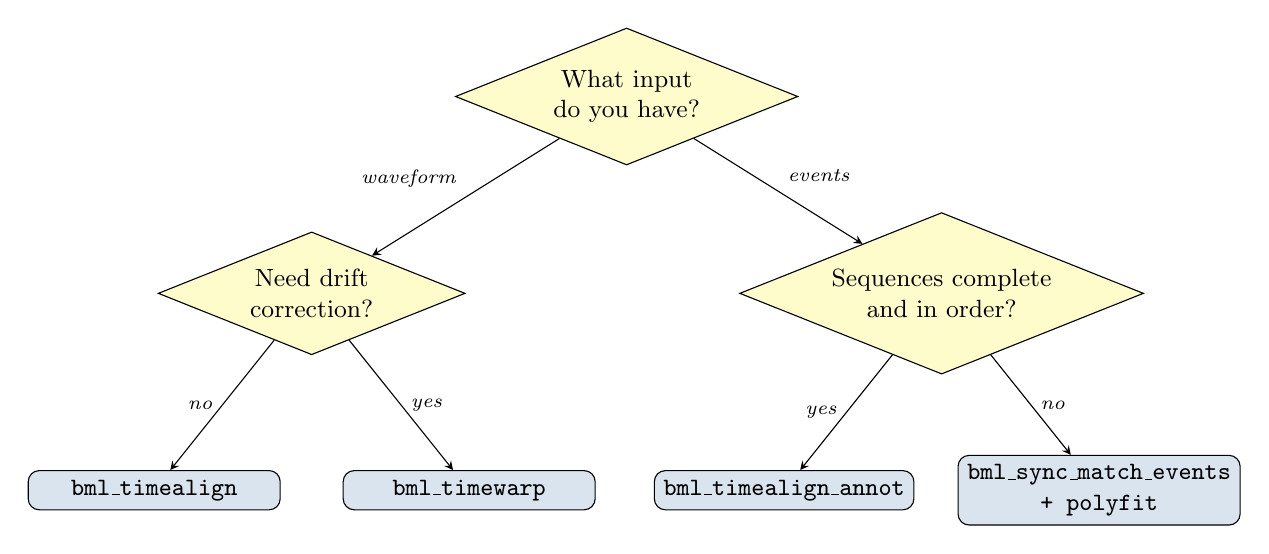
\begin{tikzpicture}[
  decision/.style={diamond, draw, fill=yellow!20, aspect=2.5, align=center, font=\small},
  result/.style={draw, rounded corners, fill=bmlblue!15, align=center, font=\small\ttfamily, minimum width=3.2cm},
  arr/.style={->, >=stealth},
  lbl/.style={font=\scriptsize\itshape}
]

\node[decision] (q1) at (0,0) {What input\\do you have?};

\node[decision] (q2) at (-4,-2.5) {Need drift\\correction?};
\node[decision] (q3) at (4,-2.5)  {Sequences complete\\and in order?};

\node[result] (r1) at (-6,-5) {bml\_timealign};
\node[result] (r2) at (-2,-5) {bml\_timewarp};
\node[result] (r3) at (2,-5)  {bml\_timealign\_annot};
\node[result] (r4) at (6,-5)  {bml\_sync\_match\_events\\+ polyfit};

\draw[arr] (q1) -- node[lbl,above left]{waveform} (q2);
\draw[arr] (q1) -- node[lbl,above right]{events} (q3);
\draw[arr] (q2) -- node[lbl,left]{no} (r1);
\draw[arr] (q2) -- node[lbl,right]{yes} (r2);
\draw[arr] (q3) -- node[lbl,left]{yes} (r3);
\draw[arr] (q3) -- node[lbl,right]{no} (r4);

\end{tikzpicture}
\end{center}

\begin{center}
\renewcommand{\arraystretch}{1.4}
\begin{tabular}{lll}
\toprule
\textbf{Situation} & \textbf{Call this} & \textbf{Why} \\
\midrule
Zoom analog click track & \texttt{bml\_sync\_analog} & shared waveform, xcorr + warp \\
Zoom audio peaks (no shared cable) & \texttt{bml\_sync\_audio\_event} & peaks → events, then grid search \\
NeuroOmega TTL pulses & \texttt{bml\_sync\_neuroomega\_event} & same signal, grid search \\
Psychtoolbox task events & \texttt{bml\_sync\_digital} & sequences may differ → DP \\
Custom: waveform, with drift & \texttt{bml\_timewarp} & \\
Custom: events, known complete & \texttt{bml\_timealign\_annot} & \\
Custom: events, possibly missing & \texttt{bml\_sync\_match\_events} & \\
\bottomrule
\end{tabular}
\end{center}

\begin{notebox}
\textbf{Why does NeuroOmega use \texttt{bml\_timealign\_annot} instead of DP?}
Both NeuroOmega and Ripple are wired to the same TTL cable, so every pulse recorded by one is also recorded by the other. The sequences are identical --- you only need to find the time shift, not figure out which event matches which. The simpler grid-search approach is sufficient and faster.

Psychtoolbox events, by contrast, travel over a potentially unreliable channel and represent a different set of event types. The DP algorithm in \texttt{bml\_sync\_match\_events} is needed to establish correspondence before estimating the offset.
\end{notebox}

% ============================================================================
\section{Event Alignment Internals: \texttt{bml\_timealign\_annot}}
\label{sec:timealign_annot}
% ============================================================================

Used by audio and NeuroOmega sync. Finds $\delta t$ (and optionally $\xi$) that minimises the total event mismatch.

\begin{formulabox}[Event alignment cost]
$\mathcal{C}(\delta t) = \sqrt{\,\displaystyle\sum_{i}\left[\min\!\left(\min_j|s_i+\delta t - m_j|,\;t_{\text{clip}}\right)\right]^2}$
\end{formulabox}

\textbf{Algorithm}: (1) brute-force scan on \texttt{linspace(-scan, scan, 2·scan/scan\_step+1)}; (2) censor outlier events with residual $>$ \texttt{censor\_mismatch}; (3) \texttt{fminsearch} refinement in 1-D (no warp) or 2-D (with warp).

% ============================================================================
\section{Continuous Signal Alignment}
% ============================================================================

\subsection{\texttt{bml\_timealign} --- cross-correlation}

\begin{enumerate}
  \item Compute scan range (max possible shift before files stop overlapping)
  \item Pad both signals to cover the scan window; resample to \texttt{resample\_freq} (10\,kHz)
  \item Preprocess: \textbf{envelope} (abs of Hilbert, downsample to 100\,Hz) or \textbf{LPF} (4th-order Butterworth)
  \item Normalize: subtract robust median, divide by robust std (16th--84th percentile)
  \item \texttt{xcorr(..., 'coeff')}, find peak lag $\to$ \texttt{slave\_delta\_t}
  \item If LPF method: also test inverted polarity; keep best
\end{enumerate}

\subsection{\texttt{bml\_timewarp} --- linear warp optimization}

\begin{formulabox}[Warp model]
$w(t) = t_{\text{pivot}} + wt_0 + (t-t_{\text{pivot}})\cdot ws_1$
\end{formulabox}

\begin{formulabox}[Warp cost function]
$\mathcal{L}(wt_0,ws_1) = -\dfrac{\langle f(w(\mathbf{t})),p\rangle}{\|f(w(\mathbf{t}_0))\|\|p\|} + \left(\dfrac{wt_0}{P_{\delta t}}\right)^{\!2} + \left(\dfrac{ws_1-1}{P_\xi}\right)^{\!4}$
\end{formulabox}

Minimised by Nelder-Mead simplex (\texttt{fminsearch}). Output: new $(s_1,t_1,s_2,t_2)$ and $\texttt{warpfactor} = 1/ws_1$.

% ============================================================================
\section{Consolidation: What It Is and Why It Matters}
\label{sec:consolidate}
% ============================================================================

\subsection{The problem consolidation solves}

After running \texttt{bml\_sync\_analog} (or any event sync), the \texttt{sync\_roi} table has \textbf{multiple rows per file} --- one per chunk. For example, a 5-minute Zoom recording synced in 3 chunks produces 3 rows, each with slightly different \texttt{(s1,t1,s2,t2)} estimates.

Before we can use these coordinates for data loading, we need to answer: do all three estimates agree? And if so, what is the \emph{single} best linear mapping for the whole file?

\begin{center}
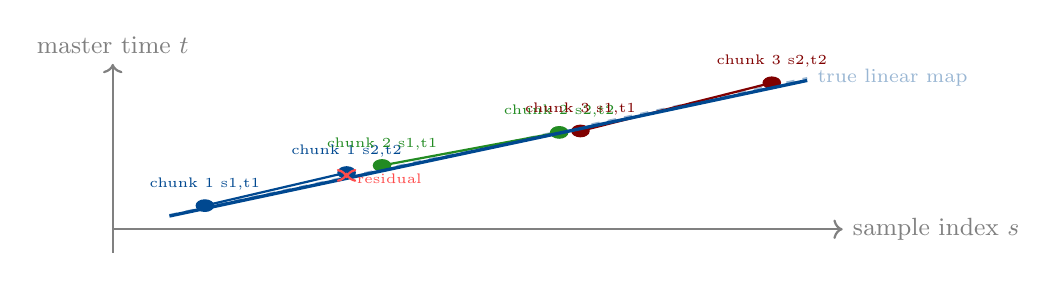
\begin{tikzpicture}[xscale=0.9, yscale=0.6]
  \draw[->, thick, gray] (-0.3,0) -- (10,0) node[right]{\small sample index $s$};
  \draw[->, thick, gray] (-0.3,-0.5) -- (-0.3,3.5) node[above]{\small master time $t$};

  % True line
  \draw[bmlblue!40, thick, dashed] (0.5, 0.3) -- (9.5, 3.2) node[right, font=\scriptsize]{true linear map};

  % Chunk 1 anchor points
  \filldraw[bmlblue] (1,0.5) circle (3.5pt) node[above=2pt, font=\tiny]{chunk 1 s1,t1};
  \filldraw[bmlblue] (3,1.2) circle (3.5pt) node[above=2pt, font=\tiny]{chunk 1 s2,t2};
  \draw[bmlblue, thick] (1,0.5)--(3,1.2);

  % Chunk 2 anchor points
  \filldraw[ForestGreen] (3.5,1.35) circle (3.5pt) node[above=2pt, font=\tiny]{chunk 2 s1,t1};
  \filldraw[ForestGreen] (6,2.05) circle (3.5pt) node[above=2pt, font=\tiny]{chunk 2 s2,t2};
  \draw[ForestGreen, thick] (3.5,1.35)--(6,2.05);

  % Chunk 3 anchor points
  \filldraw[Maroon] (6.3,2.08) circle (3.5pt) node[above=2pt, font=\tiny]{chunk 3 s1,t1};
  \filldraw[Maroon] (9,3.1) circle (3.5pt) node[above=2pt, font=\tiny]{chunk 3 s2,t2};
  \draw[Maroon, thick] (6.3,2.08)--(9,3.1);

  % Best fit line
  \draw[bmlblue, very thick] (0.5,0.28)--(9.5,3.15);

  % Residual arrows
  \draw[<->, red!70, thick] (3,1.2)--(3,1.08) node[right, font=\tiny, red!70]{residual};
\end{tikzpicture}
\end{center}

Each chunk gives two anchor points (a short line segment). If all three segments lie on the same global line (residuals $<$ 1\,ms), consolidation succeeds and we replace the three rows with one, using the global best-fit line.

\subsection{Level 1: per-file consolidation}

\begin{lstlisting}[style=matlab]
% For a file with N chunks, bml_sync_consolidate does:
% 1. Convert all (s1,s2) to raw (global) sample indices via s2raw()
i_roi = s2raw(i_roi);   % adds columns raw1, raw2

% 2. Fit a single line through all anchor points
[p, max_delta_t, off_idx] = sync_cons_group(i_roi, timewarp, 'raw');
%    p(1) = 1/Fs_eff (slope), p(2) = time intercept
%    max_delta_t = max residual in seconds

% 3. Accept or reject
if max_delta_t <= timetol   % default 1 ms
  i_roi.t1 = polyval(p, i_roi.raw1);
  i_roi.t2 = polyval(p, i_roi.raw2);
  i_roi.warpfactor = 1 ./ (i_roi.Fs .* p(1));
else
  error('consolidation failed: max residual %f ms', max_delta_t*1000);
end
\end{lstlisting}

\subsection{Level 2: contiguous file consolidation}

For devices that split recordings into consecutive files (Zoom, NeuroOmega), the same logic is applied \emph{across} files of the same type. The criterion for attempting this is that the files are contiguous in time (gap $< \texttt{timetol\_contiguous}$):

\begin{lstlisting}[style=matlab]
% Detect contiguous file groups
cfg1.criterion = @(x) ...
  (abs(sum(x.duration) - max(x.ends) + min(x.starts)) < height(x)*timetol_contiguous);
i_roi_cont = bml_annot_consolidate(cfg1, bml_roi_confluence(i_roi));

% For each contiguous group: fit one global line across all files
% After fitting, set junction times at file boundaries:
for i = 1:(height(i_roi_cont_j)-1)
  % Midpoint between adjacent anchor times = junction
  junction = (i_roi_cont_j.t2(i) + i_roi_cont_j.t1(i+1)) / 2;
  i_roi_cont_j.ends(i)     = junction;
  i_roi_cont_j.starts(i+1) = junction;
end
\end{lstlisting}

The \textbf{midpoint junction rule} ensures no gap and no overlap between adjacent files. The timing uncertainty at each file boundary is split evenly.

\subsection{What the consolidated table looks like}

\begin{lstlisting}[style=matlab]
cfg_cons = [];
cfg_cons.roi               = [sync_roi_analog; sync_roi_no; sync_roi_ptb];
cfg_cons.timetol           = 1e-3;
cfg_cons.timetol_contiguous = 1e-3;
cfg_cons.contiguous        = true;
cfg_cons.group             = 'session_id';
cfg_cons.plot_diagnostic   = true;  % shows pairwise residual matrix per file
sync_roi_final = bml_sync_consolidate(cfg_cons);
\end{lstlisting}

\begin{center}
\scriptsize
\begin{tabular}{r r r r r r r L{2.8cm} r r L{2.2cm}}
\toprule
\textbf{id} & \textbf{starts} & \textbf{ends} & \textbf{s1} & \textbf{t1} & \textbf{s2} & \textbf{t2} & \textbf{name} & \textbf{Fs} & \textbf{warpfactor} & \textbf{filetype} \\
\midrule
1 & 52310.0 & 52610.0 & 1 & 52310.000 & 9000000 & 52609.999 & session01.nev & 30000 & 1.000000 & trellis \\
2 & 52313.2 & 52612.9 & 1 & 52313.201 & 13219590 & 52612.897 & zoom\_001--3 & 44100 & 0.999998 & zoom \\
3 & 52311.7 & 52611.1 & 1 & 52311.702 & 6001200 & 52611.098 & NO\_001--2 & 20020 & 1.000003 & neuroomega \\
\bottomrule
\end{tabular}
\end{center}

\textbf{Interpreting warpfactor:} Zoom at 0.999998 means its clock ran 2\,ppm \emph{fast} (slightly fewer samples per real second than 44100). NeuroOmega at 1.000003 means its clock ran 3\,ppm \emph{slow}. Over a 5-minute session: Zoom off by 0.6\,ms, NeuroOmega off by 0.9\,ms --- easily within 1\,ms tolerance.

% ============================================================================
\section{Complete End-to-End Example}
% ============================================================================

\begin{lstlisting}[style=matlab, caption={Complete synchronization script: Trellis + Zoom + NeuroOmega + Psychtoolbox}]
%% STEP 1 -- Build initial ROI
roi = bml_roi_table(bml_info_raw(struct('folder','/data/p001/s01')));

%% STEP 2 -- Define chunks
session = bml_annot_table(table(52310, 52610, 'VariableNames',{'starts','ends'}));
session.session_id = 1;
chunks = bml_chunk_sessions(session, 3);   % 3 chunks of ~100 s

%% STEP 3 -- Analog sync: Trellis + Zoom
sync_ch = table({'trellis';'zoom'},{'ainp1';'Ch1'},{'analog';'analog'}, ...
          'VariableNames',{'filetype','channel','chantype'});
sync_ch.threshold = [NaN; NaN];

cfg_a = [];
cfg_a.roi = roi(ismember(roi.filetype,{'trellis','zoom'}),:);
cfg_a.chunks = chunks;  cfg_a.master_filetype = 'trellis';
cfg_a.sync_channels = sync_ch;
cfg_a.timewarp = true;  cfg_a.env_scan = 300;  cfg_a.lpf_scan = 1;
sync_roi_az = bml_sync_analog(cfg_a);

%% STEP 4 -- Extract master events from Trellis
master_events = bml_event2annot([], bml_read_event(roi(strcmp(roi.filetype,'trellis'),:)));
stim_events = master_events(strcmp(master_events.type,'STIM_ON'),:);

%% STEP 5 -- Event sync: NeuroOmega
cfg_no = [];
cfg_no.roi = roi(strcmp(roi.filetype,'neuroomega'),:);
cfg_no.master_events = stim_events;
cfg_no.scan = 100;  cfg_no.coarsetol = 100;  cfg_no.timewarp = false;
sync_roi_no = bml_sync_neuroomega_event(cfg_no);

%% STEP 6 -- Event sync: Psychtoolbox
ptb = bml_annot_read_tsv('sub-p001_ses-intraop_task-speech_events.tsv');
ptb_triggers = ptb(strcmp(ptb.trial_type,'STIM_ON'),:);
ptb_triggers.value = ones(height(ptb_triggers),1);

trellis_triggers = stim_events;
trellis_triggers.value = ones(height(trellis_triggers),1);

cfg_ptb = [];
cfg_ptb.timetol = 1e-3;  cfg_ptb.sim_threshold = 0.9;
cfg_ptb.weight_onset = 0.2;  cfg_ptb.onsettol = 200;
cfg_ptb.diagnostic_plot = true;
[sync_roi_ptb, hF] = bml_sync_digital(cfg_ptb, trellis_triggers, ptb_triggers);

%% STEP 7 -- Consolidate everything
cfg_cons = [];
cfg_cons.roi = [sync_roi_az; sync_roi_no];
cfg_cons.timetol = 1e-3;  cfg_cons.contiguous = true;  cfg_cons.group = 'session_id';
sync_roi_final = bml_sync_consolidate(cfg_cons);
save('/data/p001/s01/sync_roi.mat','sync_roi_final');

%% STEP 8 -- Apply PTB sync and use synchronized data
delta_t = sync_roi_ptb.delta_t(1);
warpfactor = sync_roi_ptb.warpfactor(1);
tbar = mean(ptb_triggers.starts);
ptb.starts = (ptb.starts - tbar) .* warpfactor + tbar + delta_t;
ptb.ends   = (ptb.ends   - tbar) .* warpfactor + tbar + delta_t;
% All ptb event times are now in Trellis master clock

% Load Zoom audio for a specific time window (in master time)
cfg_load = [];
cfg_load.roi = sync_roi_final(strcmp(sync_roi_final.filetype,'zoom'),:);
cfg_load.toi = [52350, 52400];   % master clock seconds
zoom_raw = bml_load_continuous(cfg_load);
\end{lstlisting}

% ============================================================================
\section{Common Pitfalls}
% ============================================================================

\begin{enumerate}[leftmargin=*, label=\textbf{\arabic*.}]
  \item \textbf{id is not stable.} Reassigned at every \texttt{bml\_annot\_table()} call. Use as a within-table label only.
  \item \textbf{The $\pm 0.5/F_s$ midpoint offset.} \texttt{t1 = starts + 0.5/Fs}, not \texttt{starts}. Forgetting this causes systematic half-sample errors.
  \item \textbf{$F_{s,\text{eff}} \neq F_s$ after warping.} Always use \texttt{bml\_idx2time}; never divide by \texttt{Fs} directly.
  \item \textbf{chunk\_extend too small.} Set \texttt{cfg.chunk\_extend} $\geq$ expected OS timestamp error (5--30\,s typical). If too small, the slave signal will not overlap the master in the extended chunk.
  \item \textbf{coarsetol too small (NeuroOmega/PTB).} If OS timestamps are off by more than \texttt{coarsetol}, the correct master events are excluded from the alignment window. Increase \texttt{coarsetol} to match the expected offset.
  \item \textbf{DP returns $>10$ chunks.} \texttt{bml\_sync\_digital} raises an error if similarity drops below \texttt{sim\_threshold} more than 10 times. This usually indicates poor event matching --- try adjusting weights or lowering \texttt{sim\_threshold}.
  \item \textbf{Consolidation failure.} A bad chunk (one where sync was unreliable) will cause the per-file polyfit to have large residuals. Use \texttt{cfg.plot\_diagnostic = true} to identify it and re-run the sync for that chunk only.
  \item \textbf{Combining analog and event sync ROI.} \texttt{bml\_sync\_analog} adds \texttt{chunk\_id} and \texttt{sync\_channel} columns; event sync functions may not. Make sure schemas match before vertically concatenating.
  \item \textbf{Warpfactor $\gg 1$ or $\ll 1$.} Values deviating from 1 by more than $10^{-4}$ (100\,ppm) are suspicious. Check whether the sync signal was clipped, noisy, or whether the wrong channel was selected.
\end{enumerate}

% ============================================================================
\section{Diagnostic Plots: How to Enable and Interpret}
\label{sec:diagnostics}
% ============================================================================

Every sync function exposes a diagnostic flag. Enable it during development and whenever a sync fails validation.

\begin{lstlisting}[language=Matlab]
cfg.diagnostic_plot = true;   % bml_sync_analog, bml_sync_neuroomega_event,
                              % bml_sync_audio_event, bml_sync_digital,
                              % bml_sync_match_events
cfg.plot_diagnostic = true;   % bml_sync_consolidate only
\end{lstlisting}

% ---------------------------------------------------------------------------
\subsection{\texttt{bml\_sync\_match\_events} --- DP similarity plot}

Produces a 2-panel figure.

\begin{figure}[H]
\centering
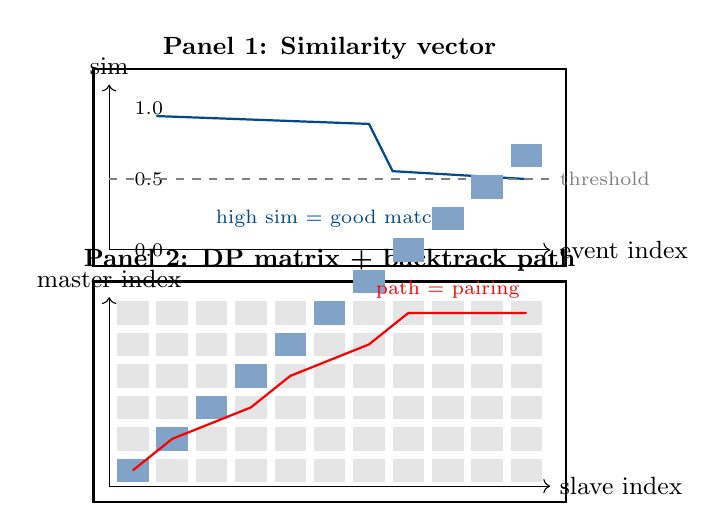
\begin{tikzpicture}[font=\small]

  % Panel 1 — similarity vector
  \draw[thick] (0,3) rectangle (6,5.5);
  \node[above] at (3,5.5) {\textbf{Panel 1: Similarity vector}};
  \draw[->] (0.2,3.2) -- (5.8,3.2) node[right] {event index};
  \draw[->] (0.2,3.2) -- (0.2,5.3) node[above] {sim};
  \node[right, font=\scriptsize] at (0.4,5.0) {1.0};
  \node[right, font=\scriptsize] at (0.4,4.1) {0.5};
  \node[right, font=\scriptsize] at (0.4,3.2) {0.0};
  % Good signal line
  \draw[bmlblue, thick] (0.8,4.9) -- (3.5,4.8) -- (3.8,4.2) -- (5.5,4.1);
  \draw[dashed, gray] (0.2,4.1) -- (5.8,4.1) node[right,font=\scriptsize,gray]{threshold};
  \node[bmlblue, font=\scriptsize, align=center] at (3,3.6) {high sim = good match};

  % Panel 2 — DP matrix
  \draw[thick] (0,0) rectangle (6,2.8);
  \node[above] at (3,2.8) {\textbf{Panel 2: DP matrix + backtrack path}};
  \draw[->] (0.2,0.2) -- (5.8,0.2) node[right] {slave index};
  \draw[->] (0.2,0.2) -- (0.2,2.6) node[above] {master index};
  % Fill DP matrix cells schematically
  \foreach \x in {0.5,1.0,1.5,2.0,2.5,3.0,3.5,4.0,4.5,5.0,5.5}{
    \foreach \y in {0.4,0.8,1.2,1.6,2.0,2.4}{
      \fill[gray!20] (\x-0.2,\y-0.15) rectangle (\x+0.2,\y+0.15);
    }
  }
  % Bright cells along diagonal
  \foreach \i/\j in {0/0,1/1,2/2,3/3,4/4,5/5,6/6,7/7,8/8,9/9,10/10}{
    \pgfmathsetmacro{\px}{0.5+\i*0.5}
    \pgfmathsetmacro{\py}{0.4+\j*0.4}
    \fill[bmlblue!50] (\px-0.2,\py-0.15) rectangle (\px+0.2,\py+0.15);
  }
  % Backtrack path
  \draw[red, thick] (0.5,0.4) -- (1.0,0.8) -- (2.0,1.2) -- (2.5,1.6) -- (3.5,2.0) -- (4.0,2.4) -- (5.0,2.4) -- (5.5,2.4);
  \node[red, font=\scriptsize] at (4.5,2.7) {path = pairing};

\end{tikzpicture}
\caption{Schematic of \texttt{bml\_sync\_match\_events} diagnostic figure.}
\end{figure}

\begin{center}
\renewcommand{\arraystretch}{1.3}
\begin{tabular}{p{5.5cm}p{8cm}}
\toprule
\textbf{Pattern} & \textbf{Meaning} \\
\midrule
All similarity values near 1 & Perfect match \\
Cluster of high values then drop & One clean matched block; use \texttt{sim\_threshold} to isolate it \\
All values $< 0.5$ & Poor match --- wrong scan range or no overlap \\
\midrule
Backtrack path is a smooth diagonal & Clean 1:1 correspondence \\
Path has horizontal/vertical runs & Events missing on one side \\
Path stays in one corner & No real overlap --- wrong files \\
\bottomrule
\end{tabular}
\end{center}

% ---------------------------------------------------------------------------
\subsection{\texttt{bml\_sync\_audio\_event} / \texttt{bml\_sync\_neuroomega\_event} --- event alignment plot}

One 2-panel figure per file: a timeline (left) and a residual histogram (right).

\begin{figure}[H]
\centering
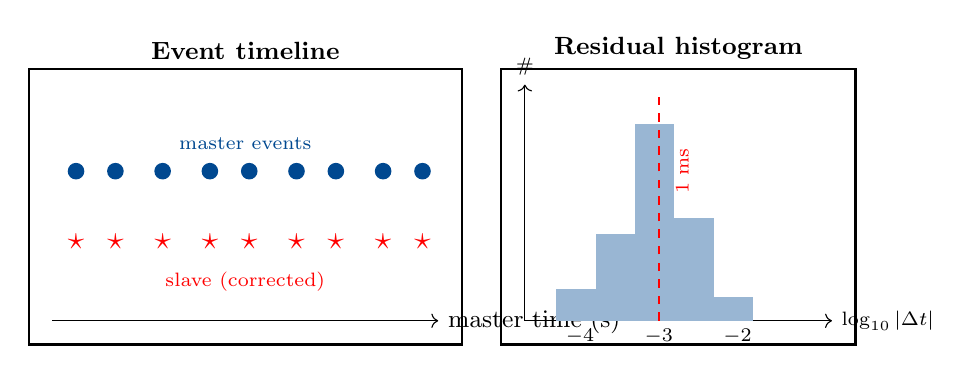
\begin{tikzpicture}[font=\small]

  % Left panel: timeline
  \draw[thick] (0,0) rectangle (5.5,3.5);
  \node[above] at (2.75,3.5) {\textbf{Event timeline}};
  \draw[->] (0.3,0.3) -- (5.2,0.3) node[right] {master time (s)};
  % Master events (blue circles)
  \foreach \x in {0.6,1.1,1.7,2.3,2.8,3.4,3.9,4.5,5.0}{
    \fill[bmlblue] (\x,2.2) circle (3pt);
  }
  \node[bmlblue, font=\scriptsize] at (2.75,2.55) {master events};
  % Slave events (red stars) — aligned
  \foreach \x in {0.6,1.1,1.7,2.3,2.8,3.4,3.9,4.5,5.0}{
    \node[red, font=\large] at (\x,1.3) {$\star$};
  }
  \node[red, font=\scriptsize] at (2.75,0.8) {slave (corrected)};

  % Right panel: histogram
  \draw[thick] (6.0,0) rectangle (10.5,3.5);
  \node[above] at (8.25,3.5) {\textbf{Residual histogram}};
  \draw[->] (6.3,0.3) -- (10.2,0.3) node[right,font=\scriptsize] {$\log_{10}|\Delta t|$};
  \draw[->] (6.3,0.3) -- (6.3,3.3) node[above,font=\scriptsize] {\#};
  % Bars (good case: peak at -3)
  \fill[bmlblue!40] (6.7,0.3) rectangle (7.2,0.7);
  \fill[bmlblue!40] (7.2,0.3) rectangle (7.7,1.4);
  \fill[bmlblue!40] (7.7,0.3) rectangle (8.2,2.8);
  \fill[bmlblue!40] (8.2,0.3) rectangle (8.7,1.6);
  \fill[bmlblue!40] (8.7,0.3) rectangle (9.2,0.6);
  \node[font=\scriptsize] at (7.0,0.1) {$-4$};
  \node[font=\scriptsize] at (8.0,0.1) {$-3$};
  \node[font=\scriptsize] at (9.0,0.1) {$-2$};
  \draw[red,dashed,thick] (8.0,0.3) -- (8.0,3.2);
  \node[red,font=\scriptsize,rotate=90] at (8.3,2.2) {1 ms};

\end{tikzpicture}
\caption{Schematic of event-alignment diagnostic. Good output: circles and stars overlap; histogram peak at $\log_{10}|\Delta t| \leq -3$ (i.e.\ $\leq 1$\,ms).}
\end{figure}

\begin{center}
\renewcommand{\arraystretch}{1.3}
\begin{tabular}{p{5.5cm}p{8cm}}
\toprule
\textbf{Pattern} & \textbf{Meaning} \\
\midrule
Circles and stars overlap & Good alignment \\
Stars consistently offset & \texttt{delta\_t} estimate slightly off; widen scan \\
Stars spread out & Residual drift; enable \texttt{timewarp = true} \\
Many extra stars & False peaks; increase \texttt{min\_rph} \\
Many circles without a star & Missed events; decrease \texttt{min\_rph} \\
\midrule
Histogram peak at $\leq -3$ ($\leq$1\,ms) & Excellent \\
Peak at $-2$ (10\,ms) & Marginal; borderline for neural data \\
Peak at $-1$ or higher & Poor; inspect timeline \\
Bimodal histogram & Matched and unmatched events mixed \\
\bottomrule
\end{tabular}
\end{center}

% ---------------------------------------------------------------------------
\subsection{\texttt{bml\_sync\_digital} --- residual + alignment plot}

One 3-panel figure per contiguous matched chunk.

\begin{figure}[H]
\centering
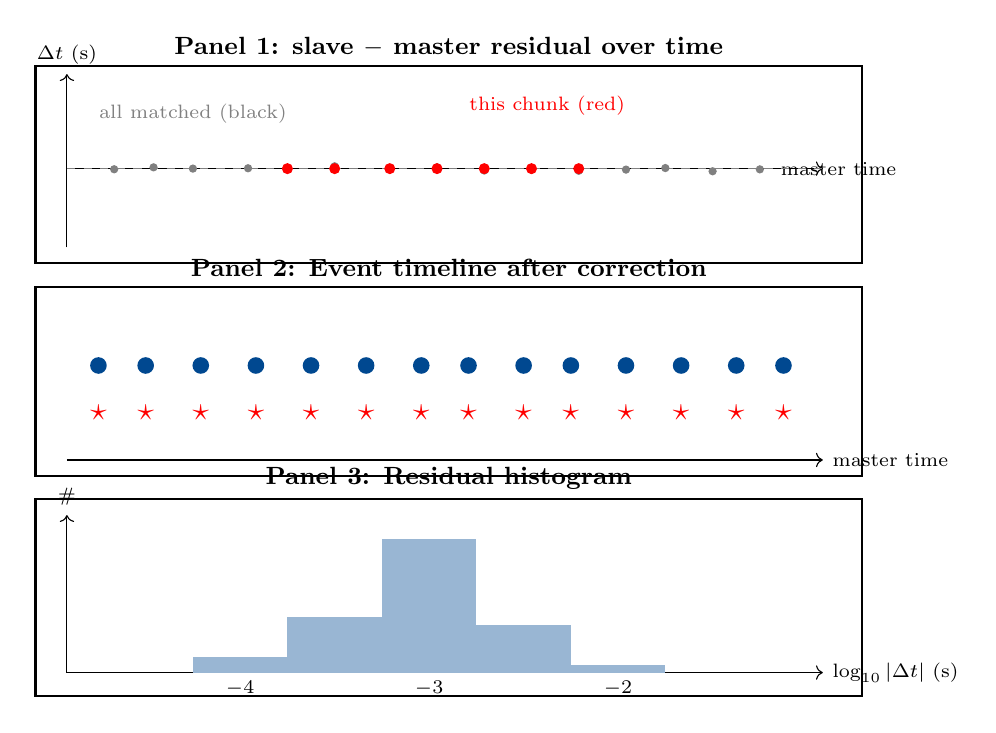
\begin{tikzpicture}[font=\small]

  % Panel 1: residual over time
  \draw[thick] (0,5.5) rectangle (10.5,8.0);
  \node[above] at (5.25,8.0) {\textbf{Panel 1: slave $-$ master residual over time}};
  \draw[->] (0.4,6.7) -- (10.0,6.7);
  \draw[->] (0.4,5.7) -- (0.4,7.9) node[above,font=\scriptsize] {$\Delta t$ (s)};
  \node[font=\scriptsize] at (10.2,6.7) {master time};
  \draw[dashed,gray] (0.4,6.7) -- (10.0,6.7);
  % All matched pairs (black dots) — slight scatter around flat line
  \foreach \x in {1.0,1.5,2.0,2.7,3.2,3.8,4.5,5.1,5.7,6.3,6.9,7.5,8.0,8.6,9.2}{
    \pgfmathsetmacro{\jitter}{0.07*(rnd-0.5)}
    \fill[black!50] (\x,{6.7+\jitter}) circle (1.5pt);
  }
  % Chunk events (red) — same flat line
  \foreach \x in {3.2,3.8,4.5,5.1,5.7,6.3,6.9}{
    \fill[red] (\x,6.7) circle (2pt);
  }
  \node[font=\scriptsize,black!50] at (2.0,7.4) {all matched (black)};
  \node[font=\scriptsize,red] at (6.5,7.5) {this chunk (red)};

  % Panel 2: timeline
  \draw[thick] (0,2.8) rectangle (10.5,5.2);
  \node[above] at (5.25,5.2) {\textbf{Panel 2: Event timeline after correction}};
  \draw[->] (0.4,3.0) -- (10.0,3.0) node[right,font=\scriptsize] {master time};
  \foreach \x in {0.8,1.4,2.1,2.8,3.5,4.2,4.9,5.5,6.2,6.8,7.5,8.2,8.9,9.5}{
    \fill[bmlblue] (\x,4.2) circle (3pt);
    \node[red,font=\large] at (\x,3.6) {$\star$};
  }

  % Panel 3: histogram
  \draw[thick] (0,0) rectangle (10.5,2.5);
  \node[above] at (5.25,2.5) {\textbf{Panel 3: Residual histogram}};
  \draw[->] (0.4,0.3) -- (10.0,0.3) node[right,font=\scriptsize] {$\log_{10}|\Delta t|$ (s)};
  \draw[->] (0.4,0.3) -- (0.4,2.3) node[above,font=\scriptsize] {\#};
  \fill[bmlblue!40] (2.0,0.3) rectangle (3.2,0.5);
  \fill[bmlblue!40] (3.2,0.3) rectangle (4.4,1.0);
  \fill[bmlblue!40] (4.4,0.3) rectangle (5.6,2.0);
  \fill[bmlblue!40] (5.6,0.3) rectangle (6.8,0.9);
  \fill[bmlblue!40] (6.8,0.3) rectangle (8.0,0.4);
  \node[font=\scriptsize] at (2.6,0.1) {$-4$};
  \node[font=\scriptsize] at (5.0,0.1) {$-3$};
  \node[font=\scriptsize] at (7.4,0.1) {$-2$};

\end{tikzpicture}
\caption{Schematic of \texttt{bml\_sync\_digital} 3-panel diagnostic. Good output: Panel 1 residuals are flat near 0; Panel 2 circles and stars overlap; Panel 3 peak at $\leq -3$.}
\end{figure}

\textbf{Panel 1 interpretation:}

\begin{center}
\renewcommand{\arraystretch}{1.3}
\begin{tabular}{p{5.5cm}p{8cm}}
\toprule
\textbf{Pattern} & \textbf{Meaning} \\
\midrule
Flat horizontal band near 0 & Pure offset, no drift --- good \\
Tilted straight line & Linear drift; enable \texttt{timewarp = true} \\
Curved or scattered & Non-linear or bad matching \\
Sudden jump & Two sessions mixed; check \texttt{cfg.group} \\
\bottomrule
\end{tabular}
\end{center}

% ---------------------------------------------------------------------------
\subsection{\texttt{bml\_sync\_consolidate} --- pairwise residual heatmap}

One $N \times N$ heatmap per file (Level 1) and per contiguous group (Level 2), where $N$ = number of chunks. Color = pairwise $\delta t$ disagreement.

\begin{figure}[H]
\centering
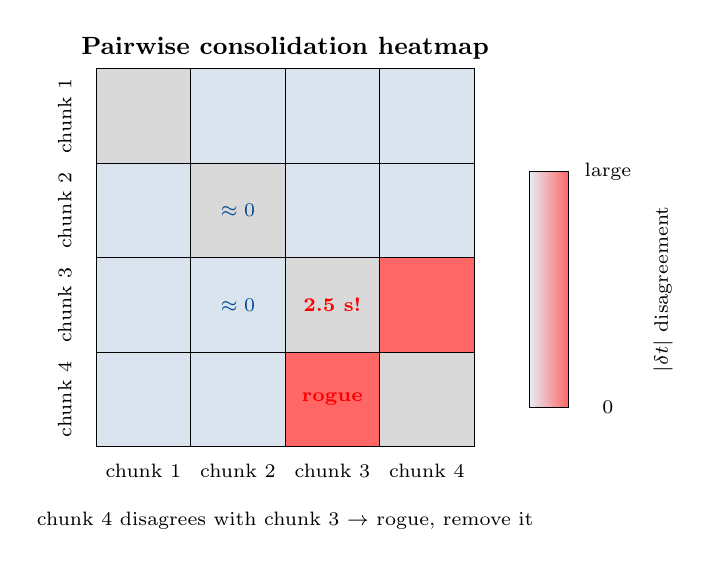
\begin{tikzpicture}[font=\small]

  \def\n{4}
  \def\cs{1.2}

  % Draw grid
  \foreach \i in {0,...,3}{
    \foreach \j in {0,...,3}{
      \pgfmathsetmacro{\isbad}{(\i==2 && \j==3) || (\i==3 && \j==2)}
      \pgfmathsetmacro{\isdiag}{\i==\j}
      \ifdim\isbad pt > 0pt
        \fill[red!60] (\j*\cs, {(3-\i)*\cs}) rectangle ({(\j+1)*\cs},{(4-\i)*\cs});
      \else
        \ifdim\isdiag pt > 0pt
          \fill[gray!30] (\j*\cs, {(3-\i)*\cs}) rectangle ({(\j+1)*\cs},{(4-\i)*\cs});
        \else
          \fill[bmlblue!15] (\j*\cs, {(3-\i)*\cs}) rectangle ({(\j+1)*\cs},{(4-\i)*\cs});
        \fi
      \fi
      \draw (\j*\cs, {(3-\i)*\cs}) rectangle ({(\j+1)*\cs},{(4-\i)*\cs});
    }
  }

  % Axis labels
  \foreach \i/\lbl in {0/1,1/2,2/3,3/4}{
    \node[font=\scriptsize] at ({\i*\cs+0.6}, -0.3) {chunk \lbl};
    \node[font=\scriptsize, rotate=90] at (-0.4, {(3-\i)*\cs+0.6}) {chunk \lbl};
  }

  % Annotations
  \node[bmlblue, font=\scriptsize] at (1.8, 3.0) {$\approx 0$};
  \node[bmlblue, font=\scriptsize] at (1.8, 1.8) {$\approx 0$};
  \node[red, font=\scriptsize\bfseries] at (3.0, 1.8) {2.5 s!};
  \node[red, font=\scriptsize\bfseries] at (3.0, 0.6) {rogue};

  % Colorbar
  \shade[left color=bmlblue!10, right color=red!60] (5.5,0.5) rectangle (6.0,3.5);
  \draw (5.5,0.5) rectangle (6.0,3.5);
  \node[font=\scriptsize] at (6.5,0.5) {0};
  \node[font=\scriptsize] at (6.5,3.5) {large};
  \node[font=\scriptsize,rotate=90] at (7.2,2.0) {$|\delta t|$ disagreement};

  \node[above, font=\small\bfseries] at (2.4,4.8) {Pairwise consolidation heatmap};
  \node[below, font=\scriptsize] at (2.4,-0.7) {chunk 4 disagrees with chunk 3 $\to$ rogue, remove it};

\end{tikzpicture}
\caption{Schematic consolidation heatmap. Blue = good agreement; red = rogue chunk. Remove the row/column that is uniformly bright and re-run consolidation.}
\end{figure}

\begin{center}
\renewcommand{\arraystretch}{1.3}
\begin{tabular}{p{5.5cm}p{8cm}}
\toprule
\textbf{Pattern} & \textbf{Meaning} \\
\midrule
All cells dark & All chunks agree --- consolidation will succeed \\
One row/column bright & That chunk is a rogue; remove and retry \\
Checkerboard & Alternating drift; shorten chunk windows \\
All cells bright & Sync failed entirely \\
\bottomrule
\end{tabular}
\end{center}

\begin{lstlisting}[language=Matlab,caption={Removing a rogue chunk and re-consolidating}]
% Find rogue chunks (>5 ms residual)
bad = sync_roi.meanerror > 0.005;
sync_roi_clean = sync_roi(~bad, :);
sync_roi_final = bml_sync_consolidate(struct('roi', sync_roi_clean));
\end{lstlisting}

% ---------------------------------------------------------------------------
\subsection{Quick-reference: what to check first}

\begin{center}
\renewcommand{\arraystretch}{1.3}
\begin{tabular}{lll}
\toprule
\textbf{Question} & \textbf{Plot} & \textbf{Panel} \\
\midrule
Did DP find the right event pairs? & \texttt{bml\_sync\_match\_events} & DP matrix path \\
Are residuals $< 1$\,ms? & Any function & Residual histogram \\
Is there drift? & \texttt{bml\_sync\_digital} & Residual over time \\
Is one chunk an outlier? & \texttt{bml\_sync\_consolidate} & Pairwise heatmap \\
Are all events accounted for? & Audio/NeuroOmega & Timeline \\
Is similarity high enough? & \texttt{bml\_sync\_match\_events} & Similarity vector \\
\bottomrule
\end{tabular}
\end{center}

% ============================================================================
\section{Best Practices and Lab Conventions}
\label{sec:bestpractices}
% ============================================================================

\subsection{Choose your sync method by signal quality}

\begin{center}
\begin{tabular}{L{4cm} L{4cm} L{5cm}}
\toprule
\textbf{Situation} & \textbf{Method} & \textbf{Why} \\
\midrule
Zoom + shared analog waveform on Trellis & Approach A: \texttt{bml\_sync\_analog} & Exploits full waveform shape; most robust \\
Zoom + only TTL click track & Approach B: \texttt{bml\_sync\_audio\_event} & Audio peaks matched to Ripple digital events \\
NeuroOmega + shared TTL & \texttt{bml\_sync\_neuroomega\_event} & TTL events present on both devices \\
Psychtoolbox / task laptop & DP matching + fallback & Clock offset can be hours; DP handles missing events \\
Session $>$ 30\,min & Enable \texttt{timewarp=true} & Drift accumulates; linear warp prevents error growth \\
\bottomrule
\end{tabular}
\end{center}

\subsection{Always validate sync quality}

Before saving or using \texttt{sync\_roi}, check:

\begin{lstlisting}[style=matlab]
% For analog sync: warpfactor should be very close to 1
assert(all(abs(sync_roi.warpfactor - 1) < 100e-6), ...
  'warpfactor deviation > 100 ppm -- check sync channel');

% For event sync: mean_sim should be high
assert(all(sync_roi.mean_sim > 0.8), ...
  'low similarity -- check event matching');

% After consolidation: residuals < 1 ms
cfg_check.timetol = 1e-3;
bml_sync_check(cfg_check, sync_roi_final);
\end{lstlisting}

\subsection{Annotation tables as the lingua franca}

Every data structure in BML is an annotation table. This is intentional:
\begin{itemize}
  \item Use \texttt{bml\_annot\_table()} to create any new table --- it enforces \texttt{id}, \texttt{starts}, \texttt{ends}, \texttt{duration} and checks for overlaps.
  \item Never store times as arrays. Always put them in a table with \texttt{starts}/\texttt{ends} so they can be filtered, joined, and validated.
  \item \texttt{bml\_annot\_filter(A, B)} is the workhorse for restricting one table to the time range of another. Use it before any alignment to avoid processing irrelevant events.
\end{itemize}

\subsection{Save intermediate outputs}

Sync is computationally expensive and hard to reproduce if session conditions change. Save:

\begin{lstlisting}[style=matlab]
save(fullfile(PATH_SYNC, 'sync_roi_final.mat'), 'sync_roi_final');
writetable(sync_roi_final, fullfile(PATH_SYNC, 'sync_roi_final.tsv'), ...
  'FileType','text','Delimiter','\t');
\end{lstlisting}

Save the \emph{un-consolidated} \texttt{sync\_roi} from each method too (analog, neuroomega, ptb). If consolidation later fails for one file, you can re-run only that step.

\subsection{The fallback-first principle}

When applying sync to event files, always prefer exact matches over interpolation (see Section~\ref{sec:ptb_fallback}). The priority order is:

\begin{enumerate}
  \item \textbf{Exact Ripple timestamp} (matched via DP): hardware-precision ground truth.
  \item \textbf{Linear warp} from the best DP-matched contiguous block: corrects offset + drift, accurate to $\sim$1--2\,ms.
  \item \textbf{No sync} (NaN): flag events that fall outside the synced session window rather than extrapolating.
\end{enumerate}

\subsection{BIDS event file conventions}

All task event logs should follow BIDS:
\begin{itemize}
  \item Columns: \texttt{onset} (seconds from task start), \texttt{duration}, \texttt{trial\_type}, \texttt{response\_time} (optional)
  \item After sync: save as \texttt{*-sync.tsv} with \texttt{starts} (master clock seconds) replacing \texttt{onset}
  \item \texttt{bml\_annot\_read\_tsv} handles the \texttt{onset}$\to$\texttt{starts} rename automatically
\end{itemize}

\subsection{Chunking strategy}

\begin{itemize}
  \item Chunk duration of 60--100\,s is a good default. Shorter chunks have less data for correlation (noisier estimates); longer chunks miss local drift changes.
  \item For long sessions ($>$2\,h), prefer 100\,s chunks with \texttt{timewarp=true}.
  \item \texttt{chunk\_extend} (extra seconds to load beyond the chunk boundary) should be at least as large as your expected OS timestamp error (typically 5--30\,s).
\end{itemize}

\subsection{Toward Python: design principles to carry forward}

The BML toolbox is currently implemented in MATLAB. The long-term goal is to migrate to Python (NumPy/Pandas/MNE). The following principles in the current design map naturally to Python:

\begin{center}
\begin{tabular}{L{4.5cm} L{4.5cm} L{4cm}}
\toprule
\textbf{MATLAB (BML)} & \textbf{Python equivalent} & \textbf{Key invariants} \\
\midrule
Annotation \texttt{table} & \texttt{pandas.DataFrame} & Always has \texttt{starts}, \texttt{ends}, \texttt{duration} columns \\
ROI table & \texttt{DataFrame} + \texttt{SyncCoords} dataclass & \texttt{s1,t1,s2,t2} define the linear map \\
\texttt{bml\_idx2time} & Pure function $\to$ \texttt{numpy} vectorized & No side effects; invertible \\
\texttt{bml\_annot\_filter} & \texttt{df[df.starts >= t0 \& ...]} & Interval overlap logic unchanged \\
\texttt{bml\_annot\_consolidate} & \texttt{groupby} + merge & Criterion function $\to$ lambda \\
DP matching & \texttt{scipy} or pure Python & Identical recurrence; only similarity function changes \\
\texttt{FT\_DATATYPE\_RAW} & \texttt{mne.io.RawArray} & Single trial, single channel for sync functions \\
\bottomrule
\end{tabular}
\end{center}

When porting, preserve the two-coordinate system \texttt{(s1,t1,s2,t2)}: it is the core abstraction that decouples sample indices from master-clock times, and nothing in the Python ecosystem provides an equivalent out of the box.

% ============================================================================
\appendix
\section{Mathematical Reference}
% ============================================================================

\subsection*{Index-to-time and inverse}
\[ F_{s,\text{eff}} = \frac{s_2-s_1}{t_2-t_1}, \qquad
   t(i) = \frac{i}{F_{s,\text{eff}}} - \frac{0.5}{F_{s,\text{eff}}} + \frac{s_2 t_1 - t_2 s_1}{s_2-s_1} \]
\[ i(t) = \mathrm{round}\!\left(\frac{t_2 s_1 - s_2 t_1 + (s_2-s_1)\,t}{t_2-t_1}\right) \]

\subsection*{Time-warp model and cost}
\[ w(t) = t_{\text{pivot}} + wt_0 + (t-t_{\text{pivot}})\cdot ws_1 \]
\[ \mathcal{L}(wt_0,ws_1) = -\frac{\langle f(w(\mathbf{t})),p\rangle}{\|f(w(\mathbf{t}_0))\|\,\|p\|}
   + \left(\frac{wt_0}{P_{\delta t}}\right)^{\!2} + \left(\frac{ws_1-1}{P_\xi}\right)^{\!4} \]
\[ t_1^{\text{new}} = t_{\text{pivot}} - wt_0 - \frac{t_2^{\text{crop}}-t_1^{\text{crop}}}{2\,ws_1}, \qquad
   t_2^{\text{new}} = t_{\text{pivot}} - wt_0 + \frac{t_2^{\text{crop}}-t_1^{\text{crop}}}{2\,ws_1} \]

\subsection*{Event alignment cost (\texttt{bml\_timealign\_annot})}
\[ \mathcal{C}(\delta t) = \sqrt{\sum_i \left[\min\!\left(\min_j |s_i+\delta t-m_j|,\;t_{\text{clip}}\right)\right]^2} \]

\subsection*{Event similarity (new 5-feature, \texttt{bml\_sync\_match\_events})}
\[ \text{sim}(\mathbf{x}_i,\mathbf{x}_j) =
   \frac{1}{W}\!\left[
   w_1\cdot\frac{1}{1+(\Delta t^\text{pre}/\tau)^2}
   + w_2\cdot\frac{1}{1+(\Delta t^\text{post}/\tau)^2}
   + w_3\cdot\mathbb{1}[v^\text{pre}_1=v^\text{pre}_2]
   + w_4\cdot\mathbb{1}[v^\text{post}_1=v^\text{post}_2]
   + w_5\cdot\frac{1}{1+((o_1-o_2)/\tau_o)^2}
   \right] \]

\subsection*{DP recurrence}
\[ \text{dp}[i{+}1,j{+}1] = \max\!\left(\text{dp}[i,j]+\text{sim}(\mathbf{x}_i,\mathbf{x}_j),\ \text{dp}[i{+}1,j],\ \text{dp}[i,j{+}1]\right) \]

\vfill
\begin{center}
{\small\color{gray}
Brain Modulation Laboratory · Massachusetts General Hospital · April 2026}
\end{center}
\end{document}
